\documentclass[a5paper, twoside, 11pt, listof=nochaptergap] {book}

%-----------------------------------------------
% packages.tex
% Package loading must be set here to ensure
% document's order
%-----------------------------------------------

% Typesetting and hyphenation helper %
\usepackage[indonesian]{babel}

% Text coloring %
\usepackage {color}

% Math typeset and equations %
\usepackage {amsmath}
\usepackage {amssymb}

% Every first paragraph is indented %
\usepackage {indentfirst}

% For enumeration and the sorts %
\usepackage {enumitem}

% For styling titles and the sorts %
\usepackage {titlesec}
\usepackage {titletoc}

% Table of Content needs %
\usepackage[titles]{tocloft}
\usepackage {tocbibind}

% For various "if" definitions %
\usepackage{etoolbox}

% Bibliography needs %
\usepackage[backend=bibtex,style=ieee,sorting=none]{biblatex}
\usepackage{url}

% Page margin %
\usepackage[top=2.5cm, bottom=2.5cm, left=2.5cm, right=2cm]{geometry}

% Paragraph alignment %
\usepackage {ragged2e}

% References debugging purpose: change 'final' to 'draft' to use %
\usepackage[final] {showkeys}

% Include pictures %
\usepackage {graphicx}
\usepackage{wrapfig}

% Code formatting %
\usepackage {listings}

% Captions formatting %
\usepackage{caption}
\usepackage{chngcntr}

% For tables need %
\usepackage{tabularx}

% Background %
\usepackage{eso-pic}

% Fonts -- compile with xelatex for correct output %
\usepackage{fontspec}

% Header-footer needs %
\usepackage{fancyhdr}

% Tables need to be rotated smh %
\usepackage{lscape}

\usepackage{hyperref}

% Subfigure %
\usepackage{subcaption}

% Float %
\usepackage{float}

\usepackage{longtable}

\usepackage{verbatim}

\usepackage[table,dvipsnames]{xcolor}

%-------------------------------------------------------------
% utils.tex
% Generic commands which may be used throughout the document
% should be set here
%-------------------------------------------------------------

%--
%	A set of command for appendix testing tables
%--


%--
%	Shortcut command for QED symbol. Use it while in math environment
%--
\newcommand{\eop}{\ensuremath{\blacksquare}}

% Bugs in LaTeX are damn AMAZING %
%--
%	Preventing \addvspace to throw error due to unended paragraph
%	#1: Usual parameter entered
%--
\let\oldaddvspace\addvspace
\renewcommand\addvspace[1]
{
	\par\oldaddvspace{#1}
}

%--
%	Preventing \contentsline to throw error due to unended paragraph
%	#1, #2, #3: Usual parameter entered
%--
\let\oldcontentsline\contentsline
\renewcommand\contentsline[3]
{
	\par\oldcontentsline{#1}{#2}{#3}
}

%--
%	Creates a text to denote an empty page
%--
\newcommand\emptypage
{
	\begin{center}
		[\textit{Halaman ini sengaja dikosongkan}]
	\end{center}
	\newpage
}

%--
%	Works as if applying two \clearpage, plus some text denoting
%	the page is empty
%--
\makeatletter
\def\cleardoublepage
{
	\clearpage
	\if@twoside
		\ifodd\c@page
			% do nothing
		\else
			\emptypage
		\fi
	\fi
}
\makeatother
%---------------------------------------------------------%
%--					Labelling Utilities					--%
%---------------------------------------------------------%

%----------- 1 Document hierarchies

%--
%	Auto label chapter with proper prefix
%	Param
%	#1: Label name. If not given, #2 will be used
%	#2:	The shown name
%--
\makeatletter

\let\oldchapter\chapter

\newcommand{\chapterstar}[1]
{
	\oldchapter*{#1}
	\protect\label{sec:#1}
}

\newcommand{\chapternostar}[2][]
{
	\ifstrempty{#1}
		{\oldchapter{#2}\protect\label{sec:#2}}
		{\oldchapter[#1]{#2}\protect\label{sec:#1}}
}
\renewcommand{\chapter}{\@ifstar{\chapterstar}{\chapternostar}}

\makeatother

%--
%	Auto label section with proper prefix
%	Param
%	#1: Label name. If not given, #2 will be used
%	#2:	The shown name
%--
\let\oldsection\section
\renewcommand\section[2][]
{
	\protect\oldsection{#2}
	\ifstrempty{#1}{\protect\label{sec:#2}}{\protect\label{sec:#1}}
}

%--
%	Auto label subsection with proper prefix
%	Param
%	#1: Label name. If not given, #2 will be used
%	#2:	The shown name
%--
\let\oldsubsection\subsection
\renewcommand\subsection[2][]
{
	\protect\oldsubsection{#2}
	\ifstrempty{#1}{\protect\label{sec:#2}}{\protect\label{sec:#1}}
}

%--
%	Auto label subsubsection with proper prefix
%	Param
%	#1: Label name. If not given, #2 will be used
%	#2:	The shown name
%--
\let\oldsubsubsection\subsubsection
\renewcommand\subsubsection[2][]
{
	\protect\oldsubsubsection{#2}
	\ifstrempty{#1}{\protect\label{sec:#2}}{\protect\label{sec:#1}}
}

%--
%	Auto label paragraph with proper prefix
%	Param
%	#1: Label name. If not given, #2 will be used
%	#2:	The shown name
%--
\let\oldparagraph\paragraph
\renewcommand\paragraph[2][]
{
	\protect\oldparagraph{#2}
	\ifstrempty{#1}{\protect\label{sec:#2}}{\protect\label{sec:#1}}
}

%----------- 2 Environment

%--
%	Environment for code listings. Used for proper labelling
%	Param
%	#1: Additional key-value pair
%	#2:	Caption name
%	#3: Label name, automatically prefixed
%--
\lstnewenvironment{code}[3][]
{
	\lstset{
		caption=#2,
		label=code:#3,
		#1
	}
}{}
%----------------------------------------------------
% styles.tex
% Things which alter how the document would look
% but not necessarily to be implemented is to be set here
%----------------------------------------------------

%--		Listing		--%
\lstdefinestyle{generic}
{
	basicstyle=\ttfamily\footnotesize,
	tabsize=2,
	numbers=left,
	numbersep=0.6em,			% distance between number and code
	numberstyle=\footnotesize\ttfamily\itshape,
	numberfirstline=false,
	xleftmargin=2.2em,		% starting margin exclusively for the code
	frame=single,			% frame type
	framexleftmargin=2.3em,	% distance between left frame to the element in the listing}
	framerule=1pt,
	breaklines=true,
	breakatwhitespace=true,
	breakindent=20pt,
	captionpos=b,
	escapechar=~
}

%--		Header-footer		--%
\fancypagestyle{normal}
{
	\fancyhf{}	% Remove all setting
	\fancyhead[LE,RO] {\thepage}
	\renewcommand {\headrulewidth}{0pt}
	\renewcommand {\footrulewidth}{0pt}
}
%------------------------------------------
% variables.tex
% All key-value pair should be set here
%------------------------------------------

% Variables declaration %
\def \kodematkul {IF184802}
\def \judul {Rancang Bangun Aplikasi Pendeteksi Daun Online pada Perangkat Bergerak Berbasis Android​}
\def \penulis {Frieda Uswatun Hasanah}
\def \oj {Sphere Online Judge}
\def \soal {Colorful Lights Party}
\def \nrp {05111540000071}
\def \jurusan {Departemen Informatika}
\def \fakultas {Fakultas Teknologi Informasi dan Komunikasi}
\def \pembimbingdua {Dwi Sunaryono S.Kom., M.Kom. }
\def \nikpembimbingdua {197205281997021001}
\def \pembimbingsatu {Dr.Eng. Radityo Anggoro , S.Kom, M.Sc.}
\def \nikpembimbingsatu {19841016 2008121002}

\def \juduleng {Design and Build of Online Leaf Detection Application on Android-Based Mobile Devices}
\def \jurusaneng {Informatics Department}
\def \fakultaseng {Faculty of Information Technology and Communication}

\def \rmk {Arsitektur dan Jaringan Komputer}
%---------------------------------------------------------
% setting.tex
% Everything that covers about the document setting
% and must be in preamble is to be implemented right here
%---------------------------------------------------------

%--		Whole document margin		--%
\setlength {\parindent}{2.5em}
\setlength {\parskip} {0.2em}

\setlist[enumerate] {itemsep=0pt, topsep=6pt, partopsep=0pt, parsep=0pt}

%--		Redactions		--%
\captionsetup[table] {skip=6pt, name={Tabel }}
\captionsetup[figure] {skip=6pt,name={Gambar }}

% Babel is weird
\addto\captionsindonesian
{
	\renewcommand {\lstlistingname}{Kode Sumber}
	\renewcommand {\chaptername}{BAB}
	\renewcommand {\contentsname}{DAFTAR ISI}
	\renewcommand {\listfigurename}{DAFTAR GAMBAR}
	\renewcommand {\listtablename}{DAFTAR TABEL}
	\renewcommand {\lstlistlistingname}{DAFTAR KODE SUMBER}
}

%--		Document hierarchy depth		--%
\setcounter{secnumdepth}{5}

%--		Document fonts		--%
\setmainfont{Times New Roman}
\setmonofont{Courier New}

%--		Set the \chapter		--%
\titleformat {\chapter}				% section
[display]							% shape
{\Centering\bfseries}				% format
{\chaptername \ \Roman{chapter}}	% label
{0.4ex}								% label-section separator
{}									% before code
[]									% after 

% for unknown reason, spacing should be set using the following format
\titlespacing*{\chapter}{0pt}{-20pt}{20pt}

%--		Set the \chapter*		--%
\titleformat {name=\chapter,numberless}	% section
[display]					% shape
{\Centering\bfseries}		% format
{}							% label
{0.4ex}						% label-section separator
{}							% before code
[]							% after

%--		Set the \section		--%
\titleformat {\section}
[hang]
{\bfseries}
{\thesection. }
{0ex}
{}
[\vspace{-0.9em}]

%--		Set the \subsection		--%
\titleformat {\subsection}
[hang]
{\bfseries}
{\thesubsection. }
{0ex}
{}
[\vspace{-0.6em}]

%--		Set the \subsubsection		--%
\titleformat {\subsubsection}
[hang]
{\bfseries}
{\thesubsubsection. }
{0ex}
{}
[\vspace{-0.6em}]

%--		Listing		--%
\lstset{style=generic}
\makeatletter
\def\lst@PlaceNumber{\ifnum\value{lstnumber}=0\else
	\llap{\normalfont\lst@numberstyle{\thelstnumber}\kern\lst@numbersep}\fi}
\makeatother

%--		Bibliography		--%
\defbibheading {bibliography}[DAFTAR PUSTAKA]{\chapter{#1}}
\urlstyle{rm}

%--		Table of Content	--%
\setlength\cftparskip{-2pt}
\setlength\cftbeforechapskip{0pt}
\setlength{\lineskip}{0pt}

% Chapter uses roman numeral
\renewcommand{\cftchapleader}{\cftdotfill{\cftdotsep}}
\newcommand{\Romannumeral}[1]{\uppercase\expandafter{\romannumeral#1}}
\renewcommand{\cftchappresnum}{\chaptername \ \Romannumeral}

% Prefix each segment
\renewcommand{\cfttabpresnum}{Tabel }
\renewcommand{\cftfigpresnum}{Gambar }

% Set each segment's indentation such that none will overlap
\cftsetindents{chapter}{0em}{4.4em}
\cftsetindents{section}{2em}{2em}
\cftsetindents{figure}{0em}{6em}
\cftsetindents{table}{0em}{5em}

%---------------------------------------------------------
%	List of how words in Indonesian should be hyphenated
%---------------------------------------------------------

% Mathematic specific
\hyphenation{kong-ru-en-si}
\hyphenation{mo-du-lo}
\hyphenation{mo-du-lus}
\hyphenation{mul-ti-pli-ca-tive}
\hyphenation{or-der}
\hyphenation{lo-ga-rit-ma dis-kret}
\hyphenation{ex-po-nent}
\hyphenation{in-vers}
\hyphenation{te-o-re-ma}
\hyphenation{lo-ga-rit-mik}
\hyphenation{lo-ga-rith-mic}
\hyphenation{pro-por-si}
\hyphenation{fak-to-ri-sa-si}
\hyphenation{kar-di-na-li-tas}
\hyphenation{po-li-no-mi-al}
\hyphenation{po-ly-no-mi-al}	
\hyphenation{stan-dar de-vi-a-si}

\hyphenation{pol-lard rho}
\hyphenation{ba-by step gi-ant step}
\hyphenation{euler to-tient func-ti-on}

% Problem specific
\hyphenation {dsa at-tack}
\hyphenation {sig-na-tu-re}
\hyphenation {run-ti-me}
\hyphenation {krip-to-gra-fi}
\hyphenation {re-pe-at-ed squ-a-ring}
\hyphenation {ge-ne-ra-tor}
\hyphenation {pu-blic}
\hyphenation {pri-va-te}
\hyphenation {key}
\hyphenation {pri-mi-ti-ve root}
\hyphenation {bru-te for-ce}
\hyphenation {ran-dom func-ti-on}
\hyphenation {step}
\hyphenation {in-te-ger o-ver-flow}
\hyphenation {mul-ti-pli-ca-ti-on}
\hyphenation {ex-po-nent-i-a-ti-on}
\hyphenation {pri-ma-li-ty}
\hyphenation {strong li-ar}
\hyphenation {pro-ba-bi-lis-tik}
\hyphenation {de-ter-mi-nis-tik}
\hyphenation {struct}
\hyphenation {po-int-er}

% Miscellaneous
\hyphenation {meng-ha-sil-kan}
\hyphenation {a-kan}
\hyphenation {ber-ja-lan}

% Cynde
\hyphenation {per-ma-sa-lah-an}
\hyphenation {pe-nge-nal-an}
\hyphenation {ko-mu-ni-ka-si}
\hyphenation {mem-per-si-ap-kan}
\hyphenation {pra-pro-ses}
\hyphenation {pseu-do-code}

% WAD
\hyphenation {me-nye-le-sai-kan}
\hyphenation {di-ker-ja-kan}
\hyphenation {di-hu-bung-kan}
\hyphenation {di-gu-na-kan}
\hyphenation {men-ja-bar-kan}
\hyphenation {me-la-ku-kan}
\hyphenation {search}

\addbibresource{bib/source.bib}

\begin{document}
	%-- Things that should go first but can't be placed in preamble
	% Figure numbering uses chapter numbering as prefix
	\counterwithin {figure}{chapter}
	
	\pagestyle {normal}
	%--
	
	\frontmatter
	\newpage
	\newgeometry{top=7cm,left=2cm,bottom=2cm}

	\sffamily
	\thispagestyle{empty}
	\color{white}
	{ \noindent TUGAS AKHIR - KI141502 }\\*[10pt] 
	{\large\textbf{\MakeUppercase{\judul}}} \\*[32pt]
	\\
	\\
	\\
	\MakeUppercase{\penulis} \\*
	NRP \nrp \\*[10pt]
	Dosen Pembimbing 1 \\*
	\pembimbingsatu \\*[10pt]
	Dosen Pembimbing 2 \\*
	\pembimbingdua \\*[10pt]
	\MakeUppercase{\jurusan} \\*
	\fakultas \\*
	Institut Teknologi Sepuluh Nopember \\*
	Surabaya, 2019
	\AddToShipoutPictureBG*{
\includegraphics[width=\paperwidth,height=\paperheight]{pembuka/img/sampul.png}}
	\rmfamily
	\normalsize
	\restoregeometry
	\color{black}
	\cleardoublepage
	
\newpage
	\newgeometry{top=7cm,left=2cm,bottom=2cm}

	\sffamily
	\thispagestyle{empty}
	{ \noindent TUGAS AKHIR - \kodematkul }\\*[10pt] 
	{\large\textbf{\MakeUppercase{\judul}}} \\*[32pt]
	\\
	\\
	\\
	\MakeUppercase{\penulis} \\*
	NRP \nrp \\*[10pt]
	Dosen Pembimbing 1 \\*
	\pembimbingsatu \\*[10pt]
	Dosen Pembimbing 2 \\*
	\pembimbingdua \\*[10pt]
	\MakeUppercase{\jurusan} \\*
	\fakultas \\*
	Institut Teknologi Sepuluh Nopember \\*
	Surabaya, 2019
	\AddToShipoutPictureBG*{
\includegraphics[width=\paperwidth,height=\paperheight]{pembuka/img/sampulWhite.png}}
	\rmfamily
	\normalsize
	\restoregeometry
	\color{black}
	\cleardoublepage

\newpage
	\newgeometry{top=7cm,left=2cm,bottom=2cm}
	\sffamily
	\thispagestyle{empty}
	{\noindent UNDERGRADUATE THESES - \kodematkul } \\*[10pt]
	{\large\textbf{\MakeUppercase{\juduleng}}} \\*[32pt]
	\\
	\\
	\\
	\\
	\MakeUppercase{\penulis} \\*
	NRP \nrp \\*[10pt]
	Supervisor 1 \\*
	\pembimbingsatu \\*[10pt]
	Supervisor 2 \\*
	\pembimbingdua \\*[10pt]
	\MakeUppercase{\jurusaneng} \\*
	\fakultaseng \\*
	Institut Teknologi Sepuluh Nopember \\*
	Surabaya, 2019
	\AddToShipoutPictureBG*{
\includegraphics[width=\paperwidth,height=\paperheight]{pembuka/img/sampulWhite.png}}
	\rmfamily
	\normalsize
	\restoregeometry
	\color{black}
	\cleardoublepage

	\chapter{LEMBAR PENGESAHAN}
\small

\begin{center}
	\textbf{\MakeUppercase\judul}
	\vspace*{0.3em}
	
	\textbf{TUGAS AKHIR} \\
	Diajukan Guna Memenuhi Salah Satu Syarat\\
	Memperoleh Gelar Sarjana Komputer\\
	pada\\
	Bidang Studi \rmk\\
	Program Studi S-1 \jurusan\\
	\fakultas \\
	Institut Teknologi Sepuluh Nopember
	
	\vspace*{0.3em}
	
	Oleh:\\
	\textbf{\penulis} \\
	NRP. \nrp
	
	\vspace*{1.1em}
\end{center}

Disetujui oleh Dosen Pembimbing Tugas Akhir: \\
\vspace*{1.3em}

\begin{tabularx}{\linewidth}{ @{}l r }
	\pembimbingsatu & ........................... \vspace*{1.4em} \\
	NIP. \nikpembimbingsatu & (Pembimbing 1) \vspace*{2.6em} \\
	
	\pembimbingdua & ........................... \vspace*{1.4em} \\
	NIP. \nikpembimbingdua & (Pembimbing 2) \vspace*{0.9em}
\end{tabularx}

\begin{center}
	\textbf {SURABAYA} \\
	\textbf {Juni 2019}
\end{center}

\normalsize
\cleardoublepage
	\chapter {ABSTRAK}

% ---- Indonesian vers.

\noindent\textbf{\MakeUppercase\judul}
\vspace*{1em}

\begin{tabularx}{\linewidth}{ l l X }
	Nama 			& : & \penulis \\
	NRP 			& :	& \nrp \\
	Departemen 		& : & \jurusan, \newline \fakultas, ITS \\
	Pembimbing I 	& : & \pembimbingsatu \\
	Pembimbing II 	& : & \pembimbingdua
	\vspace*{1em} 	% HACKY--USE ALTERNATIVE IF POSSIBLE %
\end {tabularx}

\noindent\textbf{Abstrak} \\
\itshape
\par \textit{Machine learning} atau pembelajaran mesin telah menjadi bagian dari kehidupan sehari-hari bagi banyak orang. Pengaplikasian machine learning dalam kehidupan sehari-hari termasuk dalam mendeteksi wajah, \textit{self-driving car}, prediksi cuaca, memprediksi kebiasaan orang dan banyak lagi. Banyak perusahaan, badan riset dan universitas yang terus mengembangkan \textit{machine learning} agar mendapat hasil yang lebih akurat dan cepat. Dari situlah lahir algoritma transfer, yang merupakan bagian dari \textit{machine learning}. \textit{Transfer Learning} adalah salah satu metode yang cocok digunakan untuk mengolah data yang berbentuk dua dimensi, seperti gambar dan video. 

\par Pada Tugas Akhir Ini, penulis mengusulkan untuk membuat sebuah aplikasi android yang dapat mendeteksi daun. Tujuannya adalah untuk mempermudah manusia dalam mengenali daun. Metode \textit{machine learning} yang akan digunakan adalah transfer learning, menggunakan model-model yang disediakan Keras antara lain VGG16, VGG19, MobileNet, ResNet50, Inception, dan Xception.

\vspace*{1em}
\noindent\bfseries Kata kunci: MobileNet, VGG16, ResNet50, Inception, Xception, Data Gambar, Pengenalan Daun, Aplikasi Android, Transfer Learning
\normalfont
\cleardoublepage

% ---- English vers.
\chapter {ABSTRACT}
\noindent\textbf{\MakeUppercase\juduleng}
\vspace*{1em}

\begin{tabularx}{\linewidth}{ l l X }
	Name 			& : & \penulis \\
	Student ID		& :	& \nrp \\
	Department 		& : & \jurusaneng, \newline \fakultaseng, ITS \\
	Supervisor I 	& : & \pembimbingsatu \\
	Supervisor II 	& : & \pembimbingdua
	\vspace*{1em} 	% HACKY--USE ALTERNATIVE IF POSSIBLE %
\end {tabularx}
	
\noindent\textbf{Abstract} \\
\itshape
\par Machine learning has become a part of everyday life for many people. The application of machine learning in everyday life includes face detection, self-driving car, weather prediction, predicting people's behaviour and more. Many companies, research organization and universities are continuing to develop machine learning to get more accurate and faster results. That's where the transfer algorithm is born. Transfer Learning is a part of deep learning. Transfer Learning is one method suitable for processing two-dimensional data, such as images and videos.
\par In this Thesis, the author proposes to create an android application that can detect type of leaves. The author is aiming to make it easier for humans to recognize leaves. The machine learning method that will be used is transfer learning, using the architectures provided by Keras include VGG16, VGG19, MobileNet, ResNet, Inception, and Xception.

\vspace*{1em}
\noindent\bfseries Keywords: MobileNet, VGG16, ResNet50, Inception, Xception, Image Data, Leaf Recognition, Android Applications, Transfer Learning
\normalfont
\cleardoublepage
	\chapter {KATA PENGANTAR}

Puji syukur penulis panjatkan kepada Tuhan Yang Maha Esa atas penyertaan dan karunia-Nya sehingga penulis dapat menyelesaikan tugas akhir dan laporan akhir dalam bentuk buku ini. Penelitian tugas akhir ini dilakukan untuk mengeksplorasi topik yang menarik perhatian penulis serta memenuhi salah satu syarat dalam mendapatkan gelar Sarjana Komputer di Departemen Informatika Fakultas Teknologi Informasi dan Komunikasi Institut Teknologi Sepuluh Nopember. Penulis memiliki harapan bahwa apa yang penulis kerjakan dapat membawa manfaat bagi perkembangan ilmu pengetahuan di bidang komputer dan bagi penulis sendiri selaku peneliti.

Penulis ingin mengucapkan terima kasih kepada semua pihak yang telah membimbing dan memberi dukungan baik secara langsung maupun tidak langsung selama proses pengerjaan tugas akhir ini maupun selama menempuh masa studi. Pihak tersebut antara lain:

\begin {enumerate}
	\item Tuhan yang Maha Esa, yang dengan izin dan kasihnya penulis bisa kuliah di Informatika ITS dan menyelesaikan perkuliahannya.
	\item Keluarga penulis yang telah memberikan dukungan moral, doa, dan material sehingga penulis dapat menyelesaikan Tugas Akhir ini.
	\item Bapak Dwi Sunaryono S.Kom., M.Kom. dan Bapak Dr. Radityo Anggoro S.Kom, M.Sc.  selaku pembimbing dari Tugas Akhir penulis, yang dengan bantuan dan arahan beliau penulis dapat menyelesaikan buku ini.
	\item Irsyad Rizaldi, atas dukungan dan pertemanannya selama penulis kuliah.
	\item Keluarga Pratama Ristyantika, yang terus memotivasi penulis untuk menyelesaikan tugas akhir dan menjadi teman yang dapat diandalkan.
	\item Valdi, Ade, Ipul, dan Petrus yang memberi penulis wawasan tentang dasar-dasar pembelajaran mesin.
	\item Pi, partner bridge penulis yang darinya penulis belajar banyak hal.
	\item GLBK, yang menginspirasi penulis atas keseimbangan antara prestasi dan kehidupannya.
	\item Seluruh dosen dan karyawan Departemen Informatika Fakultas Teknologi Informasi dan Komunikasi Institut Teknologi Sepuluh Nopember yang telah memberi ilmu dan waktunya untuk mempersiapkan penulis agar siap untuk masuk ke dalam dunia kerja. 
\end {enumerate}

Penulis menyadari bahwa laporan Tugas Akhir ini masih memiliki banyak kekurangan. Oleh karena itu dengan segala kerendahan hati penulis mengharapkan kritik dan saran dari pembaca untuk perbaikan penulis kedepannya. Selain itu, penulis berharap laporan Tugas Akhir ini dapat berguna bagi pembaca secara umum.

\begin{flushright}
Surabaya, Juni 2019 \\*
\vspace{5em}
\penulis
\end{flushright}
	\tableofcontents\cleardoublepage
\listoffigures\cleardoublepage
\listoftables\cleardoublepage
\lstlistoflistings\cleardoublepage
	
	\mainmatter
	\vspace{0ex}
\chapter {PENDAHULUAN}

Bab ini menjelaskan konteks tugas akhir yang akan dikerjakan, termasuk latar belakang, rumusan masalah, batasan masalah, tujuan, manfaat, metodologi, dan sistematika penulisan.

\section{Latar Belakang}
\par Teknologi informasi pada abad ini mengalami perkembangan yang pesat dan mempengaruhi hampir seluruh aspek dalam kehidupan manusia. Teknologi perangkat bergerak atau \textit{mobile device} menjadi salah satu teknologi yang saat ini banyak memunculkan inovasi - inovasi baru. Di tahun 2000, komunikasi dilakukan melalui banyak jaringan. Telepon genggam hanya bisa untuk menelepon dan menerima pesan singkat. Sekarang, pemesanan transportasi, pemesanan makanan, \textit{fintech} atau teknologi finansial, situs belanja online dan lain-lain banyak dikembangkan di perangkat bergerak.  

\par Selain teknologi berbasis perangkat bergerak, teknologi yang sedang gencar-gencarnya dikembangkan saat ini adalah \textit{Artificial Intelligence} atau Kecerdasan Buatan. Kecerdasan buatan didefinisikan sebagai kecerdasan entitas ilmiah yang dimasukkan ke dalam sebuah mesin agar dapat melakukan pekerjaan seperti yang dapat dilakukan manusia \cite{ai_def}. Beberapa macam bidang yang menggunakan kecerdasan buatan antara lain sistem pakar, permainan komputer (games), logika fuzzy, jaringan syaraf tiruan dan robotika. Pada pengolahan citra digital kecerdasan buatan juga digunakan untuk mendeteksi wajah, kebakaran, keributan dan lain-lain.
\par Pada Tugas Akhir ini, penulis akan mencoba mengimplementasikan suatu sistem untuk mengidentifikasi jenis daun berbasis android. Cara kerja aplikasi yang diusulkan adalah pengguna menangkap gambar daun dari ponsel mereka, lalu sistem akan mengirim gambar tersebut ke server. Di server gambar daun tersebut akan melalui proses klasifikasi dengan pembelajaran dalam. Metode yang akan digunakan untuk mengklasifikasi daun tersebut adalah \textit{Transfer Learning}. Kemudian hasil dari klasifikasi tersebut akan dikirim lagi ke ponsel pengguna. 
\par Penulis berharap dengan adanya aplikasi ini akan meningkatkan pengetahuan pengguna tentang manfaat daun-daun di sekitarnya.

\section {Rumusan Masalah}

Permasalahan yang akan diselesaikan pada tugas akhir ini adalah sebagai berikut:

\begin {enumerate}
\item Bagaimana mengimplementasikan \textit{transfer learning} untuk mendeteksi jenis daun? 
\item Bagaimana mengembangkan sebuah aplikasi berbasis android yang mengirim gambar ke server dan menerima balasan berupa jenis daun?
\item Bagaimana melakukan proses klasifikasi daun pada server?
\item Arsitektur \textit{transfer learning} mana yang lebih akurat dalam mendeteksi jenis daun? 
\end {enumerate}

\section {Batasan Masalah}

Batasan masalah yang terdapat pada Tugas Akhir ini adalah sebagai berikut : 
\begin {enumerate}
\item Implementasi program menggunakan bahasa pemrograman Java untuk Android serta \textit{backend} dan Python untuk mendeteksi daun. 
\item Implementasi aplikasi android untuk mengirim gambar daun ke server dan menampilkan balasan berupa jenis daun.
\item Android yang digunakan minimal API 21 atau Lollipop versi 5.0
\item Sistem pengenalan daun dirancang untuk deteksi satu daun dalam satu gambar. 
\item Dataset diperoleh dari https://archive.ics.uci.edu/ml/datasets/leaf yang ditambahkan dengan dataset dari penulis sendiri. 
\end {enumerate}

\section {Tujuan}

Tujuan pembuatan Tugas Akhir ini adalah merancang aplikasi pendeteksi daun online berbasis perangkat bergerak android. 

\section{Manfaat}
Dengan adanya Tugas Akhir ini, diharapkan dapat memberikan manfaat kepada pengguna perangkat bergerak berbasis android sebagai aplikasi mobile yang memberikan informasi mengenai jenis daun. 

\section {Metodologi}

Metodologi pengerjaan yang digunakan pada tugas akhir ini memiliki beberapa tahapan. Tahapan-tahapan tersebut adalah sebagai berikut:

\begin{enumerate}
\item Penyusunan proposal tugas akhir\\
Tahapan awal dari Tugas Akhir ini adalah penyusunan Proposal Tugas Akhir yang berisi pendahuluan, deskripsi dan gagasan metode-metode yang dibuat dalam Tugas Akhir ini.
Pendahuluan ini terdiri dari latar belakang diajukannya Tugas Akhir, rumusan masalah dan batasan masalah yang ditetapkan, serta manfaat dari hasil pembuatan Tugas Akhir ini. Selain itu, dijabarkan pula tinjauan pustaka yang digunakan sebagai referensi pendukung pembuatan Tugas Akhir. Terdapat pula sub bab jadwal kegiatan yang menjelaskan jadwal pengerjaan Tugas Akhir.
\item Studi literatur\\
Pada tahap ini dilakukan pencarian literatur berupa jurnal yang digunakan sebagai referensi untuk pengerjaan tugas akhir ini. Literatur yang dipelajari pada pengerjaan tugas akhir ini
berasal dari jurnal ilmiah yang diambil dari berbagai sumber di internet, serta berbagai literatur online tambahan terkait Keras dan Android.
\item Implementasi Perangkat Lunak\\
Pada tahap ini akan dilaksanakan implementasi metode dan algoritma yang telah direncanakan. Implementasi sistem menggunakan Python 3 sebagai bahasa pemrograman,
TensorFlow dan Keras sebagai framework, serta library pendukung lainya. Untuk aplikasi android sistem akan menggunakan bahasa pemrograman Java.
\item Pengujian dan Evaluasi\\
Tahap pengujian dan evaluasi dilakukan menggunakan dataset Daun untuk mengetahui hasil dan performa arsitektur yang telah dibangun. Evaluasi dilakukan dengan metode pengukuran akurasi.
\item Penyusunan buku\\
Pada tahap ini dilakukan penyusunan buku yang menjelaskan seluruh konsep, teori dasar dari metode yang digunakan, implementasi, serta hasil yang telah dikerjakan sebagai dokumentasi dari pelaksanaan Tugas Akhir.
\end{enumerate}

\section {Sistematika Penulisan}

Sistematika laporan tugas akhir yang akan digunakan adalah sebagai berikut:

\begin{enumerate}
\item Bab 1 : PENDAHULUAN

Bab ini menjelaskan konteks tugas akhir yang akan dikerjakan, termasuk latar belakang, rumusan masalah, batasan masalah, tujuan, manfaat, metodologi, dan sistematika penulisan.

\item Bab 2 : TINJAUAN PUSTAKA

Bab ini berisi kajian teori dari metode dan algoritma yang digunakan dalam penyusunan Tugas Akhir ini. Secara garis besar, bab ini berisi tentang Android, Transfer Learning dan library yang digunakan.

\item Bab 3 :  PERANCANGAN SISTEM

Bab ini berisi pembahasan mengenai perancangan dari metode Transfer Learning yang digunakan untuk pengenalan ekspresi daun pada data gambar.

\item Bab 4 : IMPLEMENTASI

Bab ini membahas implementasi dari perancangan yang telah dibuat pada bab sebelumnya. Penjelasan berupa kode yang digunakan untuk proses implementasi.

\item Bab 5 : PENGUJIAN DAN EVALUASI

Bab ini membahas tahapan uji coba, kemudian hasil uji coba dievaluasi terhadap kinerja dari sistem yang dibangun.

\item Bab 6 : KESIMPULAN DAN SARAN

Bab ini merupakan bab yang menyampaikan kesimpulan dari hasil uji coba yang dilakukan, masalah-masalah yang dialami pada proses dan tertulis saat pengerjaan Tugas Akhir, dan saran untuk  pengembangan solusi kedepannya.

\end{enumerate} \cleardoublepage
	\chapter {TINJAUAN PUSTAKA}
Bab ini membahas mengenai teori-teori dasar yang digunakan dalam Tugas Akhir. Teori-teori tersebut diantaranya adalah \textit{Transfer Learning}, \textit{Server} dan beberapa teori lain yang mendukung pembuatan Tugas Akhir. Penjelasan ini bertujuan untuk memberikan gambaran umum dan diharapkan dapat mendukung sistem yang dibangun.

\section{Android}
Android menyediakan kerangka kerja aplikasi yang kaya dan memungkinkan Anda membangun aplikasi dan game inovatif untuk perangkat seluler di lingkungan bahasa pemrograman Java.   Android merupakan sistem operasi perangkat bergerak yang berbasis linux kernel dan merupakan open-source. Android dikembangkan oleh Google.

\par Perangkat keras yang mendukung Android terutama didasarkan pada platform arsitektur ARM. Ada sekitar 2,6 juta aplikasi yang dikembangkan untuk Android. Android mengandalkan Linux versi 2.6 untuk layanan sistem inti seperti keamanan, manajemen memori, manajemen proses, tumpukan jaringan, dan model driver. 

\par Komponen-komponen dalam platform Android antara lain : linux kernel, lapisan abstraksi perangkat keras, native c++ dan \textit{android runtime}, kerangka kerja Java API, dan sistem aplikasi \cite{android_def}.


\section{Transfer Learning}
\par Transfer Learning adalah sebuah riset masalah pada pembelajaran mesin yang terfokus pada menyimpan pengetahuan yang didapat ketika menyelesaikan suatu masalah dan mengaplikasikannya ke masalah yang berbeda namun berhubungan \cite{transfer_def}. Transfer Learning akan berfungsi dengan baik apabila fitur-fitur pada permasalahan awal bersifat umum dan bukan spesifik sehingga model yang dihasilkan dapat digunakan kembali pada permasalahan yang sejenis.
\begin{figure}[!ht]
	\centering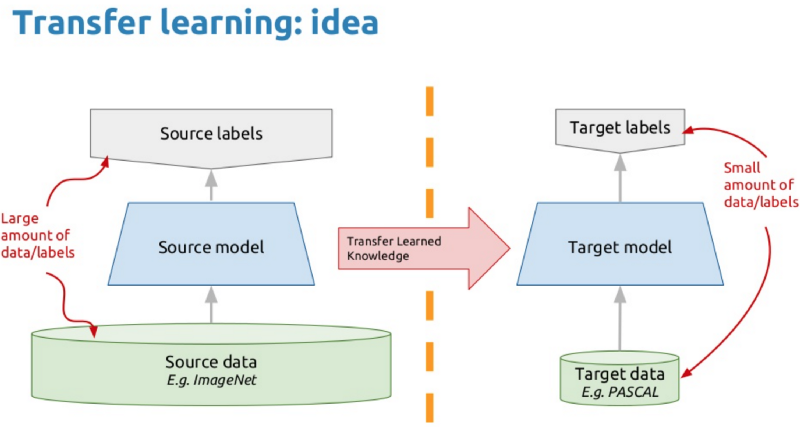
\includegraphics[width=0.8\textwidth]{bab2/figures/transfer-works.png}
	\caption{Diagram alir transfer learning\cite{transfer_pic}}
	\label{fig:transfer-works}
\end{figure}
\par Pendekatan Transfer Learning adalah dengan tiga metode, yaitu : 

\subsection{Melatih Sebuah Model untuk Menggunakannya Kembali}
\par Ketika kita ingin menyelesaikan Task A namun tidak memiliki cukup data untuk melatihnya dengan Deep Neural Network. Di sisi lain kita memiliki Task B dimana kita bisa melatihnya dengan Deep Neural Network. Maka kita dapat melatih Task B dengan Deep Neural Network dan menggunakannya sebagai titik awal dalam menyelesaikan Task A.

\subsection{Menggunakan Pre-Trained Model}
\par Pendekatan kedua adalah menggunakan dengan menggunakan pre-trained model atau model yang telah dilatih sebelumnya. Di internet banyak yang menyediakan pre-trained model ini, salah satunya Keras. Keras merupakan sebuah library pada Python yang menyediakan berbagai pre-trained model seperti VGG16, VGG19, XCeption, MobileNet dan lain-lain. 

\subsection{Ekstraksi Fitur}
\par Pendekatan lain adalah menggunakan algoritma \textit{Deep Learning} untuk menemukan representasi terbaik dari permasalahan. Pendekatan ini sering juga disebut \textit{Representation Learning}.  Cara menggunakan pendekatan ini adalah dengan menemukan fitur apa saja yang paling menggambarkan permasalahan kita. 
\par Meskipun metode Deep Learning dapat mengekstrak fitur secara otomatis, kita harus menentukan fitur mana saja yang ingin dimasukkan dalam \textit{Network}. Representasi yang sudah dipelajari kemudian dapat digunakan untuk menyelesaikan permasalahan lain juga. Metode ini cocok untuk menyelesaikan permasalahan Visi Komputer karena dapat mengurangi ukuran data set yang kemudian mengurangi waktu komputasi juga\cite{transfer_how}.

\begin{figure}[ht]
	\centering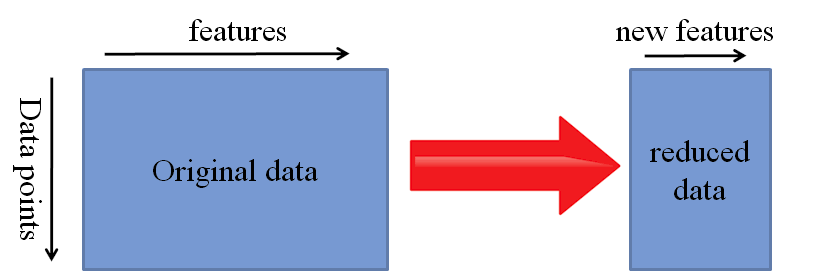
\includegraphics[width=0.7\textwidth]{bab2/figures/rep_features.png}
	\caption{Pembelajaran Representasi\cite{transfer_how}}
	\label{fig:rep-works}
\end{figure}

\section{Server}
\par Server dapat merujuk baik pada perangkat keras atau perangkat lunak yang menyediakan layanan tertentu kepada pengguna. Jika merujuk pada perangkat keras, server digunakan untuk menyimpan semua data. Sedangkan pada sisi perangkat lunak, fungsi server adalah sebagai pusat kontrol untuk memproses permintaan yang diterima dari browser.

\par Secara sederhana, server bekerja atas permintaan dari sebuah klien. Misalnya saja untuk kasus web server, ketika Anda mengetikkan suatu alamat website menggunakan browser, maka artinya komputer Anda sedang bertindak sebagai klien yang meminta informasi kepada web server. Web server tersebut kemudian mengirimkan isi website ke komputer Anda, sehingga Anda pun dapat mengakses isi website tersebut.

\par Untuk kasus lainnya, seperti server FTP, mungkin agak sedikit berbeda. Pada server FTP, Anda dapat mengunggah sebuah dokumen atau data menuju server FTP, sehingga dapat disimpan dalam server tersebut. Sebagai klien, Anda berhak untuk menyimpan data Anda di server FTP. Nantinya, jika ada orang lain yang tergabung dalam jaringan server tersebut dan ingin mengunduh data atau dokumen Anda, maka server FTP akan menyediakan koneksi untuk klien lain tersebut.

\par Sebuah perangkat komputer yang dijadikan server biasanya dirancang sedikit berbeda dari komputer – komputer klien. Dalam hal spesifikasi perangkat dan juga dalam hal sistem operasi misalnya, spesifikasi perangkat komputer yang digunakan sebagai server harus dibuat tinggi (karena harus menangani lalu lintas data yang cukup besar), sedangkan sistem operasinya harus menggunakan sistem operasi khusus server seperti Windows Server atau pun Linux Ubuntu Server / Linux Mint Server\cite{server_def}.

\section{Python}
\par Python adalah bahasa pemrograman yang populer. Python sering dimanfaatkan dalam pengembangan web, perangkat lunak, penelitian, dan system scripting. Python dapat digunakan untuk menangani data besar dan melakukan operasi matematika yang kompleks. Python bekerja di berbagai platform seperti Windows, Mac, Linux, Raspberry Pi, dan lain-lain. Python dirancang untuk mudah dibaca, yaitu memiliki sintaks yang sederhana dan
menggunakan bahasa Inggris\cite{python_def}.
Penulis menggunakan Python dalam Tugas Akhir ini karena tersedianya library pembelajaran mesin dan pembelajaran dalam yang lengkap pada bahasa pemrograman ini.


\section{Tensorflow}
\par TensorFlow adalah library \textit{open source} untuk pembuatan program yang membutuhkan komputasi numerik berkinerja tinggi. Dibuat oleh tim Google Brain, TensorFlow adalah librari \textit{open-source} untuk komputasi numerik dan pembelajaran mesin skala besar. Tensorflow menggunakan Python untuk menyediakan API front-end yang nyaman untuk membangun aplikasi dengan kerangka kerja, sambil mengeksekusi aplikasi tersebut dalam C++.TensorFlow menyediakan fungsi-fungsi \textit{machine learning} dan \textit{deep learning}, dan dapat dijalankan dalam CPU atau GPU\cite{tensorflow_def}.

\section{Keras}
\par Keras adalah API \textit{neural network} tingkat tinggi, ditulis dengan Python dan mampu berjalan di atas TensorFlow, CNTK, atau Theano. Keras dikembangkan dengan fokus pada mempercepat eksperimen\cite{keras_def}.
\par Keras tidak melakukan operasi tingkat rendahnya sendiri, seperti produk tensor dan konvolusi. Keras bergantung pada back-end. Meskipun Keras mendukung beberapa back-end, back-end utamanya adalah TensorFlow, dan pendukung utamanya adalah Google. 
\par Keras API dikemas dalam TensorFlow sebagai tf.keras, yang seperti yang disebutkan sebelumnya akan menjadi TensorFlow API utama pada TensorFlow 2.0.

\section{ImageNet}
\par ImageNet adalah sebuah proyek yang bertujuan untuk memberi label dan mengkategorikan gambar ke dalam 22.000 kategori objek berbeda untuk riset Visi Komputer. Model-model dilatih pada lebih dari 1,2 juta gambar untuk pelatihan dengan 50.000 gambar validasi dan 100.000 gambar uji\cite{vgg19_def}.

\section{VGG16} 
\par VGG16 (juga disebut OxfordNet) adalah arsitektur jaringan saraf convolutional yang dinamai Grup Visual Geometry dari Oxford, yang mengembangkannya.VGG16 terdiri dari 3 x 3 layer konvolusi, 2 x 2 max layer, dan fully-connected layer. Total layer pada VGG16 adalah 16\cite{vgg16_def}.

\par Untuk menghitung layer konvolusi, matriks 3x3 pada input data gambar dibaca dari kiri atas ke kanan bawah. 
Pada setiap posisi gambar, dihasilkan sebuah angka yang merupakan dot product antara bagian gambar tersebut dengan filter yang digunakan. Dengan menggeser \textit{(convolve)} filter di setiap kemungkinan posisi filter pada gambar, dihasilkan sebuah activation map.

\par Proses ini diulang dengan beberapa filter berbeda, hingga menghasilkan “gambar” baru yang merupakan kumpulan dari activation maps.

\par Pooling layer adalah lapisan yang mengurangi dimensi dari feature map atau lebih dikenal dengan langkan untuk downsampling, sehingga mempercepat komputasi karena parameter yang harus diupdate semakin sedikit dan mengatasi overfitting. Pooling yang biasa digunakan adalah Max Pooling dan Average Pooling. Max Pooling untuk menentukan nilai maksimum tiap pergeseran filter, sementara Average Pooling akan menentukan nilai rata-ratanya.
\begin{figure}[!ht]
	\centering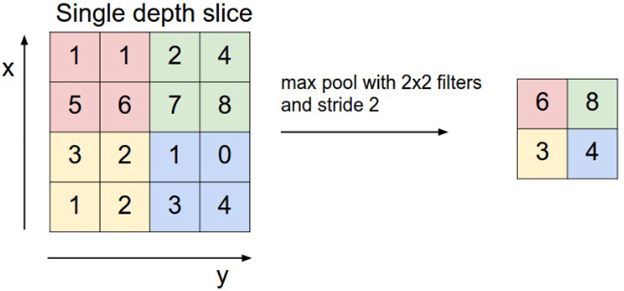
\includegraphics[width=0.7\textwidth]{bab2/figures/max pooling.png}
	\caption{Contoh dari Max Pooling\cite{max_pool}}
	\label{fig:abstraksi1}
\end{figure}


\section{VGG19}
\par VGG-19 adalah jaringan saraf convolutional yang dilatih pada lebih dari satu juta gambar dari database ImageNet. Jaringan ini memiliki 19 lapisan dan dapat mengklasifikasikan gambar ke dalam 1000 kategori objek, seperti keyboard, mouse, pensil, dan banyak binatang. Akibatnya, jaringan telah mempelajari representasi fitur yang kaya untuk berbagai gambar. Jaringan memiliki ukuran input gambar 224 x 224\cite{imagenet_def}.
\begin{figure}[!ht]
	\centering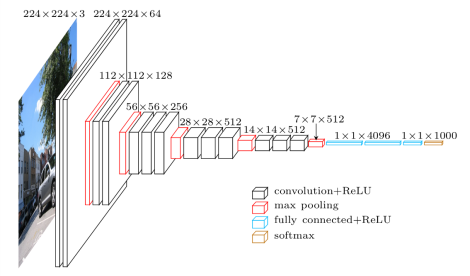
\includegraphics[width=0.7\textwidth]{bab2/figures/figure-vgg.png}
	\caption{Visualisasi dari arsitektur VGG\cite{figure_vgg}}
	\label{fig:abstraksi1}
\end{figure}

\par Kelebihan VGG16 dan VGG19 antara lain jumlah layernya yang dapat dianggap \textit{deep}, relatif mudah untuk dijelaskan dibanding arsitektur lain. Kekurangan dari VGG16 dan VGG19 yaitu sangat lama untuk proses pelatihan,dan ukuran yang sangat besar yaitu 533 MB untuk VGG16 dan 574 MB untuk VGG19.


\section{MobileNet}
\par MobileNet didasarkan pada arsitektur ramping yang menggunakan konvolusi \textit{depth-wise} terpisah untuk membangun jaringan saraf yang dalam dan ringan\cite{mobilenet_def}. Keunggulan dari MobileNet adalah kompleksitas yang lebih kecil dan ukuran yang lebih kecil juga. Dengan kompleksitas yang lebih kecil, kekurangan dari MobileNet adalah akurasinya yang tidak setinggi arsitektur yang lebih kompleks. Berikut ini adalah gambar dari cara kerja \textit{depth-wise separable convolution} pada MobileNet.

\begin{figure}[!ht]
	\centering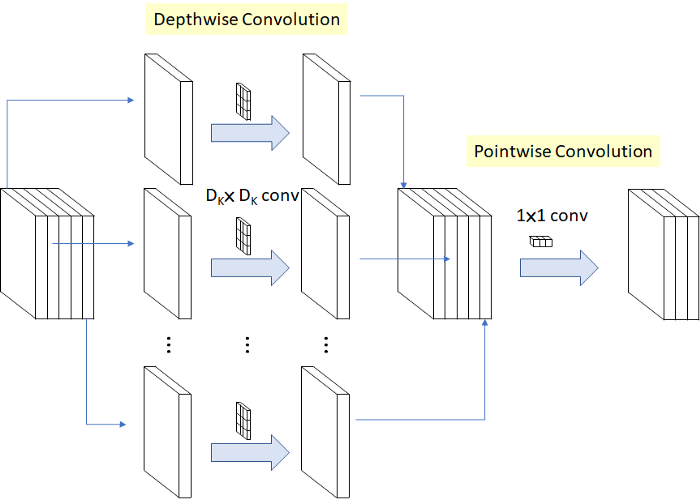
\includegraphics[width=0.7\textwidth]{bab2/figures/mobilenet.png}
	\caption{\textit{Depth-Wise Separable Convolution pada MobileNet}\cite{mobilenet_def}}
	\label{fig:abstraksi1}
\end{figure}

\section{ResNet50}
\par ResNet adalah singkatan dari Residual Network. Residual dapat dipahami sebagai pengurangan fitur yang dipelajari dari input layer tersebut\cite{resnet_def}. Karena hal ini, ResNet merupakan arsitektur yang dalam dengan jumlah layer mencapai 200. ResNet yang akan dipakai oleh penulis adalah ResNet50, yang berarti Residual Network dengan jumlah layer 50. Meskipun jumlah layer pada ResNet lebih banyak daripada VGG16 atau VGG19, ukuran modelnya lebih kecil karena penggunaan pooling global rata-rata dan bukan fully-connected layer. Ukuran ResNet50 adalah 102 MB.

\section{InceptionV3}
\par Tujuan dari modul Inception adalah untuk bertindak sebagai "ekstraktor fitur multi-level" dengan menghitung konvolusi 1×1, 3×3, dan 5×5 dalam modul jaringan yang sama - output dari filter ini kemudian ditumpuk bersama dimensi channel dan dimasukkan ke lapisan berikutnya dalam jaringan.

\par Inkarnasi asli dari arsitektur ini disebut GoogLeNet, tetapi manifestasi selanjutnya hanya disebut Inception vN di mana N mengacu pada nomor versi yang dikeluarkan oleh Google.

\par InceptionV3 memiliki 42 layer, namun ukurannya lebih rendah dari VGG, yaitu 96 MB.

\begin{figure}[!ht]
	\centering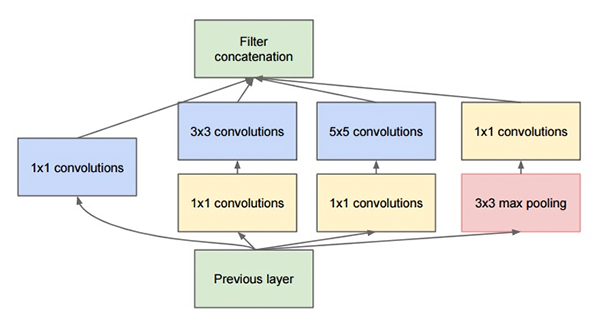
\includegraphics[width=0.7\textwidth]{bab2/figures/inception.png}
	\caption{Inception Model\cite{inception}}
	\label{fig:abstraksi1}
\end{figure}
\section{Xception}
\par Xception diciptakan oleh pembuat dan kepala pengelola Keras yaitu Francois Chollet. Xception sama seperti Inception, hanya saja modul standar Inception digantikan oleh \textit{depth-wise separable convolution}. Keunggulan dari Xception adalah ukuran arsitekturnya yang paling kecil yaitu 91 MB\cite{xception}.


\section{Logistic Regression}
\par Logistic Regression digunakan dalam ilmu biologi pada awal abad kedua puluh. Itu kemudian digunakan dalam banyak aplikasi ilmu sosial. Logistic Regression digunakan ketika target adalah kategorikal.

\begin{figure}[!ht]
	\centering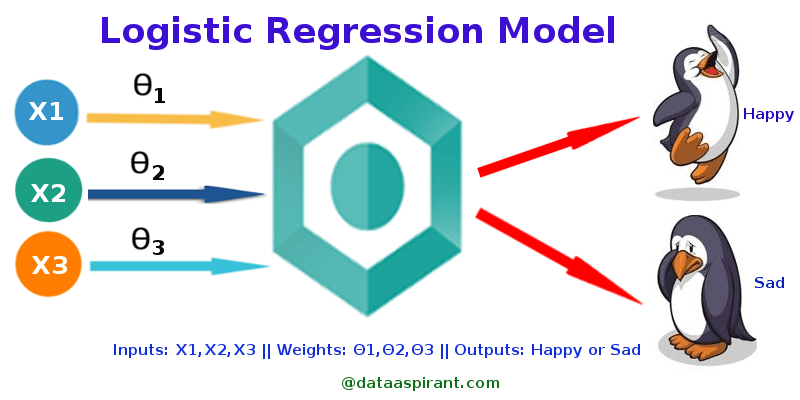
\includegraphics[width=0.9\textwidth]{bab2/figures/logistic.png}
	\caption{Visualisasi dari Logistic Regression\cite{logistic_def}}
	\label{fig:abstraksi1}
\end{figure}
\section{Precision}
\par Precision didefinisikan sebagai jumlah benar positif dibagi dengan jumlah benar positif ditambah jumlah salah positif. Salah positif adalah kasus-kasus yang oleh modelnya salah diberi label sebagai positif yang sebenarnya negatif\cite{precisionrecall}.

\section{Recall}
\par Recall adalah jumlah benar positif dibagi jumlah benar positif dibagi jumlah salah negatif \cite{precisionrecall}. Salah negatif menunjukkan nilai di mana kelas aktual adalah ya tetapi kelas prediksi adalah tidak. Misalnya, jika kelas aktual mengatakan bahwa akan hujan tetapi kelas prediksi menunjukkan bahwa tidak akan ada hujan.

\section{F1 Score}
\par Penghitungan F1 Score adalah dengan cara mengalikan dua dengan precision dan recall kemudian dibagi dengan penjumlahan precision dan recall. F1 Score mungkin merupakan ukuran yang lebih baik untuk digunakan jika kita perlu menemukan keseimbangan antara Precision dan Recall dan ada distribusi kelas yang tidak rata\cite{f1score_def}.

\begin{figure}[!ht]
	\centering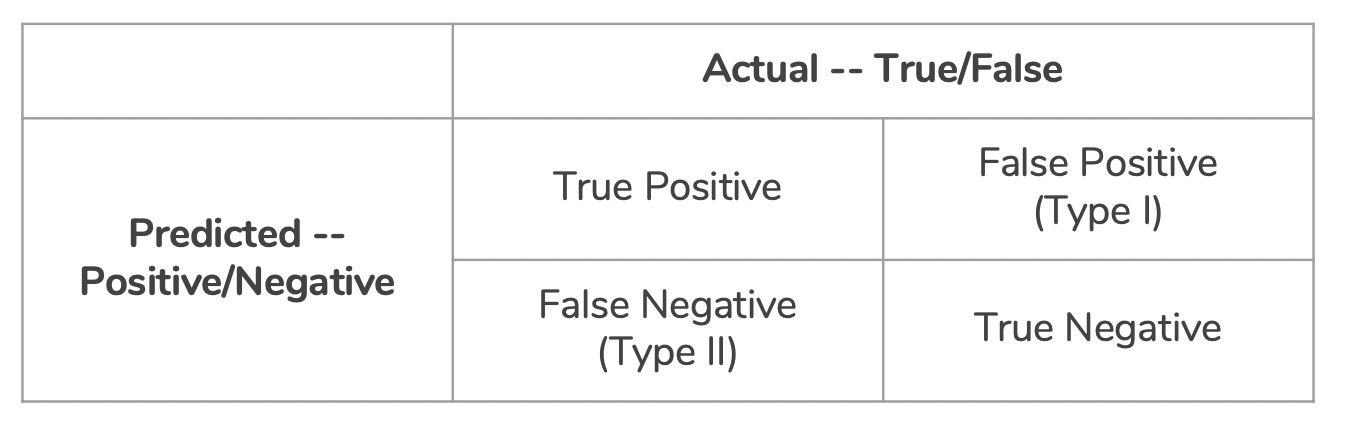
\includegraphics[width=0.9\textwidth]{bab2/figures/confusion.png}
	\caption{\textit{Confusion Matrix}\cite{precisionrecall}}
	\label{fig:conf}
\end{figure}

\begin{figure}[!ht]
	\centering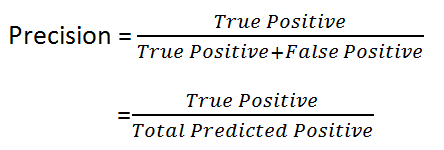
\includegraphics[width=0.7\textwidth]{bab2/figures/precision.png}
	\caption{Rumus\textit{ Precision}\cite{precisionrecall}}
	\label{fig:conf}
\end{figure}

\begin{figure}[!ht]
	\centering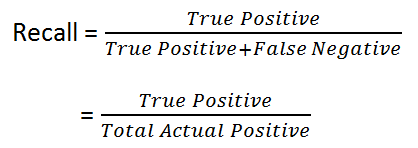
\includegraphics[width=0.7\textwidth]{bab2/figures/recall.png}
	\caption{Rumus\textit{ Recall}\cite{precisionrecall}}
	\label{fig:conf}
\end{figure}

\begin{figure}[!ht]
	\centering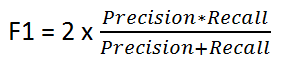
\includegraphics[width=0.7\textwidth]{bab2/figures/f1.png}
	\caption{Rumus \textit{F1 Score}\cite{precisionrecall}}
	\label{fig:conf}
\end{figure}

\section{Spring}
\par Spring adalah sebuah kerangka kerja yang bersifat \textit{open-source}. Spring sendiri pertama kali dibuat oleh Rod Johnson tahun 2002 sebagai alternatif dari Java Enterprise Edition yang bertujuan untuk mengatasi masalah desain sistem dalam pengembangan aplikasi enterprise. Selain itu, Spring juga mengimplementasikan beberapa teknologi IoC (\textit{Inversion of Control}) dan DI (\textit{Dependency Injection}) ke dalam sebuah MVC \textit{(Model View Controller})\cite{spring_def}.  \cleardoublepage
	\chapter{PERANCANGAN SISTEM}

Bab ini menjelaskan mengenai perancangan data dan sistem rancang bangun aplikasi pendeteksi daun berbasis Android. Bab ini juga akan menjelaskan gambaran umum sistem.

\section{Perancangan Data}
\par Data yang digunakan sebagai masukan awal dari sistem rancang bangun aplikasi pendeteksi daun berbasis Android adalah dataset yang dibuat Pedro F. B. Silva dan Andra Marasal menggunakan spesimen Rubim Almeida da Silva dari the Faculty of Science, University of Porto, Portugal. Dataset tersebut berisi 483 data yang terbagi dalam 40 kelas. 

\begin{figure}[ht]
	\begin{subfigure}{0.5\textwidth}
		\centering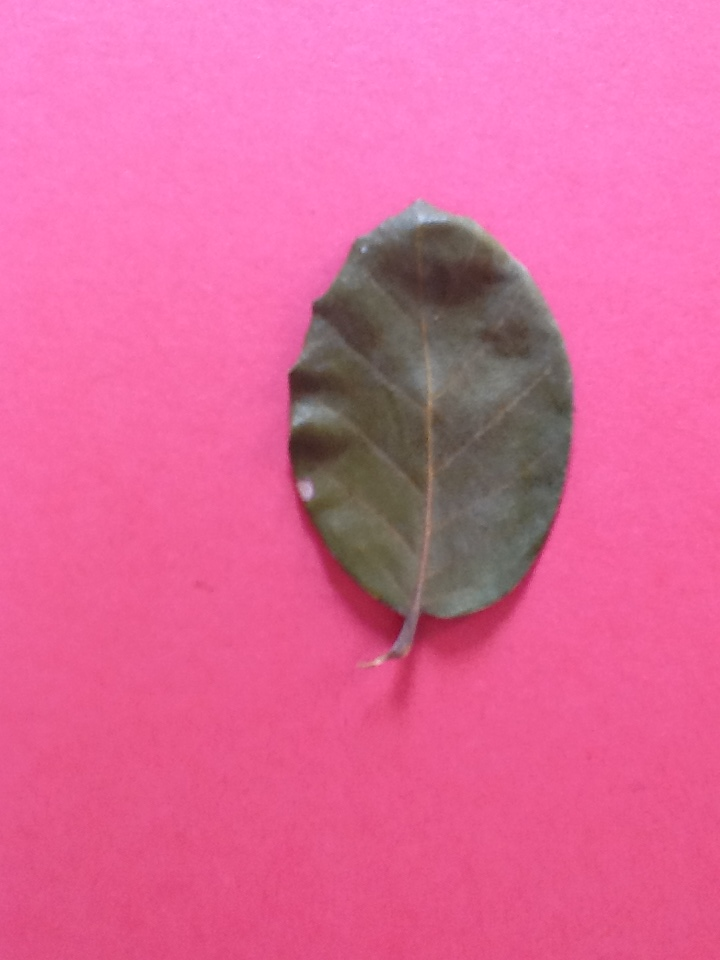
\includegraphics[width=\linewidth]{bab3/figures/quercus_suber.JPG}
		\caption{Quercus Suber}
		\label{fig:quercus_suber}
	\end{subfigure}
	~
	\begin{subfigure}{0.5\textwidth}
		\centering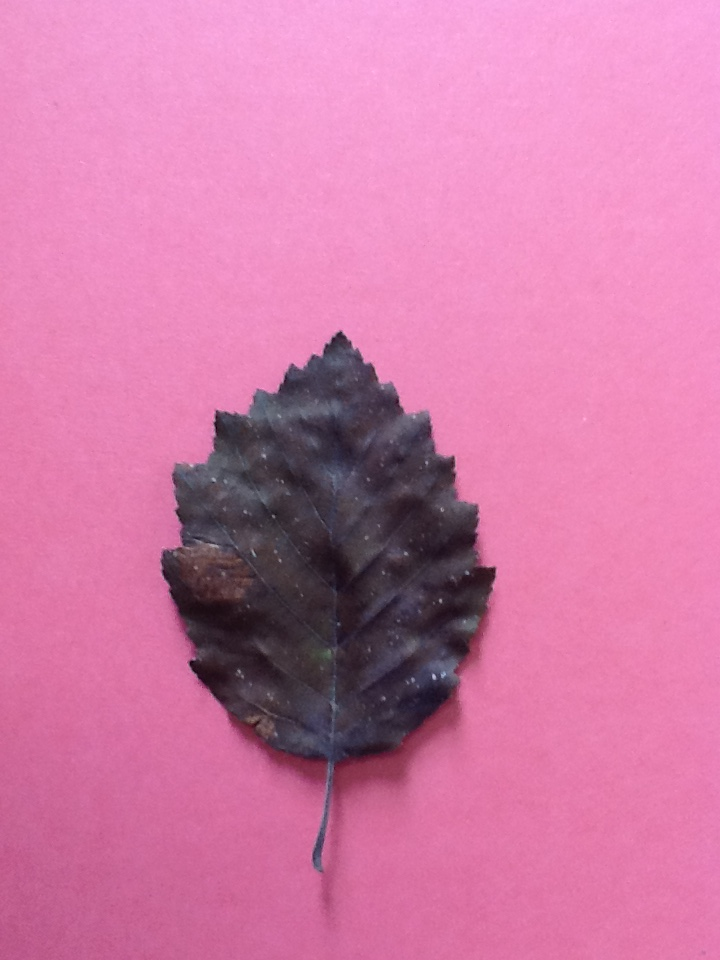
\includegraphics[width=\linewidth]{bab3/figures/alnus_sp.JPG}
		\caption{Alnus sp}
		\label{fig:alnus_sp}
	\end{subfigure}
	~
	\caption{Contoh gambar daun pada dataset}
\end{figure}

\par Dataset tersebut berisi gambar sehelai daun dengan background pink dan tidak ada benda lain di sekelilingnya. 

\par Selain dataset dari Pedro F. B. Silva dan Andra Marasal, penulis akan menambahkan dataset sendiri dengan daun-daun yang umum ditemukan di Indonesia. Adapun gambar-gambar yang akan ditambahkan penulis lebih tidak teratur dalam artian latar belakangnya bisa berwarna-warni dan mengandung noise.

\section{Desain Umum Sistem}
\par Desain umum dari sistem pendeteksi daun berbasis Android ini terdiri dari tiga bagian, yaitu tahap ekstraksi fitur, tahap pelatihan, dan aplikasi Android. 
\par Tahap ekstraksi fitur dilakukan paling awal dalam tahap membuat model. Gambar diekstraksi fiturnya dengan menggunakan arsitektur-arsitektur yang akan diuji dan dibandingkan. Setelah fitur-fitur pada gambar diekstraksi dan disimpan dalam file, dilakukan tahap pelatihan. 
\par Dengan tahap pelatihan, dibuatlah sebuah model atau \textit{classifier} yang akan dipakai untuk memprediksi daun yang diunggah ke-server.
\par Pengguna sendiri akan berinteraksi dengan perangkat lunak berbasis android yang memiliki beberapa fungsi, seperti prediksi, unggah dan latih. Aplikasi Android akan berperan sebagai perantara antara pengguna dan peladen.

\subsection{Tahap Ekstraksi Fitur}
\par Sistem dan model \textit{deep learning} adalah arsitektur berlapis yang mempelajari fitur yang berbeda pada layer yang berbeda (representasi hierarkis fitur berlapis). Layer-layer ini akhirnya terhubung ke lapisan terakhir (biasanya \textit{fully-connected layer}, untuk mendapatkan hasil akhir. Arsitektur berlapis ini memungkinkan kita untuk menggunakan jaringan yang sudah dilatih sebelumnya (seperti InceptionV3 atau VGG) tanpa layer terakhirnya sebagai ekstraktor fitur tetap untuk tugas-tugas lain.
\par Ini idealnya digunakan ketika data yang kita coba latih sangat mirip dengan pre-trained model dan ukuran dataset kecil.
\par Pada tahap awal dari ekstraksi fitur dilakukan praproses input menggunakan library Keras. Bobot pre-trained yang tersedia di Keras dilatih dengan langkah preproses yang didefinisikan dalam fungsi \textit{preprocess input} yang tersedia untuk setiap arsitektur jaringan (VGG16, InceptionV3, dll).
\par Setelah praproses dilakukan, akan dijalankan ekstraksi fitur dengan arsitektur jaringan tertentu. Setelah fitur diekstraksi, hasil ekstraksi fitur tersebut  akan di-\textit{flatten} sehingga membentuk array. Lalu setelah fitur dari semua gambar telah diekstraksi, datanya disimpan dalam file berekstensi h5. Label-label dari gambar-gambar tersebut juga akan disimpan dalam file berekstensi h5. File-file h5 ini akan digunakan dalam tahap selanjutnya yaitu pembuatan model.

\subsubsection{Ekstraksi Fitur dengan VGG16}
\par VGG16 merupakan arsitektur konvolusi pembelajaran dalam dengan bobot 16 layer, yang terdiri dari 12 \textit{Convolutional Layer}, 3 \textit{Fully-Connected Layer}, dan \textit{Softmax Layer}. Proses ekstraksi fitur ini dilakukan menggunakan metode FCN (Fully Convolutional Layer) VGG-16. Dimana nilai vector yang di dapatkan dari Ekstraksi Fitur dengan 13 \textit{Convolution Layer}, 5 \textit{Max Pooling Layer} yang telah diubah menjadi vector menggunakan fungsi Flatten akan dijadikan sebagai input atribut data untuk tahap pembentukkan model.

\subsubsection{Ekstraksi Fitur dengan VGG19}
\par VGG19 adalah arsitektur dengan bobot 19 layer, terdiri dari 16 Convolution Layer dan 5 Max Pooling Layer. Secara garis besar VGG19 mirip dengan VGG16. 

\subsubsection{Ekstraksi Fitur dengan MobileNet}
\par Arsitektur ini menggunakan \textit{depth-wise separable convolution}yang secara signifikan mengurangi jumlah parameter bila dibandingkan dengan jaringan dengan konvolusi normal dengan kedalaman yang sama dalam jaringan. Ini menghasilkan jaringan saraf yang dalam dan ringan. 
\par Pengurangan jumlah parameter secara signifikan mengurangi jumlah total operasi yang menguntungkan dalam aplikasi \textit{mobile} dengan daya komputasi yang lebih sedikit.

\subsubsection{Ekstraksi Fitur dengan ResNet50}
\par ResNet-50 adalah jaringan saraf convolutional yang dilatih pada lebih dari satu juta gambar dari basis data ImageNet. Jaringan ini memiliki kedalaman 50 lapisan dan dapat mengklasifikasikan gambar ke dalam 1000 kategori objek, seperti keyboard, mouse, pensil, dan banyak binatang. Akibatnya, jaringan telah mempelajari representasi fitur yang kaya untuk berbagai gambar. Jaringan memiliki ukuran input gambar 224x224.

\par ResNet menggunakan \textit{skip connection} untuk menambahkan output dari lapisan sebelumnya ke lapisan selanjutnya. Ini membantu mengurangi masalah gradien yang hilang dan memungkinkan untuk melakukan pembelajaran dalam dengan banyak layer.

\subsubsection{Ekstraksi Fitur dengan InceptionV3}
\par InceptionV3 merupakan arsitektur jaringan yang terdiri dari 48 layer. InceptionV3 juga dilatih menggunakan lebih dari sejuta gambar pada basis data ImageNet. Inception menumpuk konvolusi 5x5 menjadi dua konvolusi 3x3 untuk peningkatan performa.

\subsubsection{Ekstraksi Fitur dengan Xception}
\par Xception diusulkan oleh François Chollet sendiri, pencipta dan kepala pengelola Keras.Xception adalah perpanjangan dari arsitektur Inception yang menggantikan modul Inception standar dengan \textit{depth-wise convolution}. Xception menampilkan serialisasi terkecil dengan berat hanya 91MB.

\subsection{Tahap Pelatihan}
\par Apabila ekstraksi fitur dengan arsitektur yang dipilih telah selesai, saatnya untuk melakukan pelatihan. Pelatihan dilakukan untuk membangun model klasifikasi untuk mendeteksi daun. 
\par Pelatihan dimulai dengan membuka file-file hasil ekstraksi fitur. Kemudian dari data hasil ekstraksi fitur tersebut dipecah menjadi train dataset dan test dataset untuk validasi. Ukuran perbandingan dari data test dan data train dapat diatur di file konfigurasi. Setelah dilakukan penyesuaian atau fit antara data train dengan metode klasifikasi \textit{Logistic Regression}. Untuk setiap data test akan dilakukan prediksi yang kemudian dicatat hasil keseluruhannya pada file berekstensi txt.
\par Hasil dari pengujian model akan di evaluasi menggunakan variabel evaluasi precision, recall,dan f1-score. 

\subsection{Aplikasi Android}
\par Aplikasi Android ini dikembangkan dengan bahasa pemrograman Java dan \textit{Integrated Development Environment} Android Studio. Adapun aplikasi ini akan membutuhkan akses pada kamera ponsel dan internet untuk dijalankan. Untuk menjalankan kamera pada ponsel, akan digunakan library fotoapparat. Terdapat tiga fitur pada aplikasi Android, yaitu :
\begin {enumerate}
\item Upload
\par Pengguna dapat mengunggah foto-foto daun, untuk menambah dataset pada server. Dengan fitur ini diharapkan jumlah label dan dataset daun bertambah, yang meningkatkan kredibilitas aplikasi. 
\par Fitur upload akan menembak API pada server dengan parameter gambar daun yang telah diubah menjadi string serta nama daun.
\item Predict
\par Pengguna dapat mengunggah foto daun yang ingin dicari jenisnya. Server kemudian akan mengirim hasil prediksi daun pada ponsel pengguna.
\par Fitur predict akan menembak API pada server dengan parameter gambar yang telah diubah menjadi bentuk string.
\item Train
\par Pengguna menembak API pada server yang men-\textit{trigger} server untuk menjalankan pelatihan ulang pada model.
\end {enumerate}\begin{flushleft}
	
\end{flushleft}
 \cleardoublepage
	\chapter {IMPLEMENTASI}

\section{Lingkungan Implementasi}

Lingkungan implementasi dan pengembangan menggunakan sebuah komputer dengan spesifikasi perangkat lunak dan perangkat keras sebagai berikut.

\begin{enumerate}
	\item Perangkat Keras
	\par Implementasi tugas akhir ini menggunakan desktop personal computer ASUS X555Q. Namun digunakan untuk menjalankan Google Colab dengan spesifikasi :
	\begin{enumerate}
		\item GPU: 1x Tesla K80 , having 2496 CUDA cores, compute 3.7, 12GB(11.439GB Usable) GDDR5 VRAM
		\item CPU: 1x single core hyper threaded i.e(1 core, 2 threads) Xeon Processors @2.3Ghz (No Turbo Boost) , 45 MB Cache
	\end{enumerate}
	\item Perangkat Lunak
	\begin{enumerate}
		\item Sistem Operasi Linux 18.04 64-bit
		\item Android Studio
		\item Bahasa Pemrograman Java
		\item Bahasa Pemrograman Python
		\item Library Keras
	\end{enumerate}
\end{enumerate}

\section{Implementasi Ekstraksi Fitur}
Subbab ini menjabarkan implementasi ekstraksi fitur. 

\begin{lstlisting}[language=java, caption=Konfigurasi, label=code:config, firstnumber=1]
{
"model"           : "mobilenet",
"weights"         : "imagenet",
"include_top"     : false,

"train_path"      : "../RGB",
"test_path"		  : "test",
"features_path"   : "mobilenet/features.h5",
"labels_path"     : "mobilenet/labels.h5",
"results"         : "mobilenet/results.txt",
"classifier_path" : "mobilenet/classifier.pickle",
"model_path"	  : "mobilenet/model",

"test_size"       : 0.3,
"seed"            : 9,
"num_classes"     : 42
}
\end{lstlisting}
\par Konfigurasi yang dapat diatur antara lain nama model, bobot, train path atau direktori folder yang akan dilatih, features path atau direktori file untuk menyimpan fitur, label path atau direktori file untuk menyimpan label, test size atau perbandingan rasio antara data test dan data train, results atau direktori file untuk menyimpan hasil train keseluruhan. 
\begin{lstlisting}[language=python, caption=Membaca konfigurasi, label=code:open_config, firstnumber=37]
	with open('conf/conf.vgg19.json') as f:
	config = json.load(f)
	
	model_name = config["model"]
	weights = config["weights"]
	include_top = config["include_top"]
	train_path = config["train_path"]
	features_path = config["features_path"]
	labels_path = config["labels_path"]
	test_size = config["test_size"]
	results = config["results"]
	model_path = config["model_path"]
\end{lstlisting}
\par Fungsi untuk membaca konfigurasi dari file berbentuk json. 

\begin{lstlisting}[language=python, caption=Menentukan arsitektur untuk ekstraksi fitur, label=code:choose_architecture, firstnumber=58]
if model_name == "vgg16":
base_model = VGG16(weights=weights)
model = Model(inputs=base_model.input, outputs=base_model.get_layer('fc1').output)
image_size = (224, 224)

elif model_name == "vgg19":
base_model = VGG19(weights=weights)
model = Model(input=base_model.input, output=base_model.get_layer('fc1').output)
image_size = (224, 224)

elif model_name == "resnet50":
base_model = ResNet50(weights=weights)
lastLayer = base_model.layers[-2]
model = Model(input=base_model.input, output=lastLayer.output)  # base_model.get_layer('custom').output)
image_size = (224, 224)

elif model_name == "inceptionv3":
base_model = InceptionV3(include_top=include_top, weights=weights, input_tensor=Input(shape=(299, 299, 3)))
output = base_model.output
model = Model(inputs=base_model.input, outputs=output)  # base_model.get_layer('custom').output)
image_size = (299, 299)

elif model_name == "mobilenet":
base_model = MobileNet(include_top=include_top, weights=weights, input_tensor=Input(shape=(224, 224, 3)),
input_shape=(224, 224, 3))
output = base_model.output
model = Model(inputs=base_model.input, outputs=output)  # base_model.get_layer('custom').output)
image_size = (224, 224)
elif model_name == "xception":
base_model = Xception(weights=weights)
model = Model(input=base_model.input, output=base_model.get_layer('avg_pool').output)
image_size = (299, 299)
else:
base_model = None
\end{lstlisting}
\par Fungsi untuk menentukan arsitektur apa yang akan digunakan untuk mengekstraksi fitur dari file konfigurasi json.

\begin{lstlisting}[language=python, caption=Preproses Data, label=code:preprocess, firstnumber=123]
count = 1
for i, label in enumerate(train_labels):
cur_path = train_path + "/" + label
count = 1
for image_path in glob.glob(cur_path + "/*.JPG"):
img = image.load_img(image_path, target_size=image_size)
x = image.img_to_array(img)
x = np.expand_dims(x, axis=0)
x = preprocess_input(x)
feature = model.predict(x)
flat = feature.flatten()  ### double flatten dg diatas
features.append(flat)
labels.append(label)
print("[INFO] processed - " + str(count))
count += 1
print("[INFO] completed label - " + label)
\end{lstlisting} 

\par Fungsi untuk melakukan preproses pada data gambar dan mengekstraksi fiturnya menggunakan arsitektur yang telah dipilih.

\begin{lstlisting}[language=python, caption=Menyimpan hasil ekstraksi fitur, label=code:save_h5, firstnumber=149]
h5f_data = h5py.File(features_path, 'w')
h5f_data.create_dataset('dataset_1', data=np.array(features))

h5f_label = h5py.File(labels_path, 'w')
h5f_label.create_dataset('dataset_1', data=np.array(le_labels))

h5f_data.close()
h5f_label.close() 
\end{lstlisting}

\par Fungsi untuk menyimpan hasil ekstraksi fitur beserta labelnya masing-masing kedalam file berekstensi h5.

\section{Implementasi Pelatihan}
\par Berikut adalah implementasi sumber kode untuk melakukan pelatihan dari data yang sudah diekstraksi. 

\begin{lstlisting}[language=python, caption=Membaca file hasil ekstraksi fitur, label=code:read_h5, firstnumber=34]
h5f_data  = h5py.File(features_path, 'r')
h5f_label = h5py.File(labels_path, 'r')

features_string = h5f_data['dataset_1']
labels_string   = h5f_label['dataset_1']

features = np.array(features_string)
labels   = np.array(labels_string)

h5f_data.close()
h5f_label.close()
\end{lstlisting}

Fungsi untuk membaca hasil dari ekstraksi fitur yang disimpan dalam file h5. Hasilnya kemudian diubah kebentuk numpy array dan file h5 ditutup.

\begin{lstlisting}[language=python, caption=Membagi data test dan data train, label=code:train_test_split, firstnumber=52]
(trainData, testData, trainLabels, testLabels) = train_test_split(np.array(features),
np.array(labels),
test_size=test_size,
random_state=seed)
\end{lstlisting}

\par Melakukan pembagian dataset menjadi data train dan data test yang rasionya dapat diatur pada file konfigurasi.

\begin{lstlisting}[language=python, caption=Penyesuaian dengan \textit{Logistic Regression}, label=code:logistic, firstnumber=65]
model = LogisticRegression(random_state=seed)
model.fit(trainData, trainLabels)
\end{lstlisting}
\par Menggunakan metode klasifikasi \textit{Logistic Regression} untuk mempelajari hubungan antara data dan label untuk memprediksi hasil uji di tahap berikutnya.

\begin{lstlisting}[language=python, caption=Melakukan Prediksi Probabilitas, label=code:predict_proba, firstnumber=74]
for (label, features) in zip(testLabels, testData):
# predict the probability of each class label and
# take the top-5 class labels
predictions = model.predict_proba(np.atleast_2d(features))[0]
predictions = np.argsort(predictions)[::-1][:5]

# rank-1 prediction increment
if label == predictions[0]:
rank_1 += 1

# rank-5 prediction increment
if label in predictions:
rank_5 += 1

rank_1 = (rank_1 / float(len(testLabels))) * 100
rank_5 = (rank_5 / float(len(testLabels))) * 100

f.write("Rank-1: {:.2f}%\n".format(rank_1))
f.write("Rank-5: {:.2f}%\n\n".format(rank_5))

\end{lstlisting}
\par Fungsi untuk menghitung akurasi dari prediksi probabilitas rank-1 dan rank-5. Yang dimaksud rank-1 adalah apabila hasil prediksi pertama atau yang probabilitasnya paling tinggi. Yang dimaksud rank-5 adalah lima hasil prediksi dengan probabilitas tertinggi. Apabila hasil prediksi sama dengan label, variabel rank-1 bertambah. Apabila label ada di rank-5, variabel rank-5 bertambah.

\begin{lstlisting}[language=python, caption=Menyimpan model dan hasil, label=code:save_model, firstnumber=105]
# evaluate the model of test data
preds = model.predict(testData)

# write the classification report to file
f.write("{}\n".format(classification_report(testLabels, preds)))
f.close()

# dump classifier to file
pickle.dump(model, open(classifier_path, 'wb'))

\end{lstlisting}

\par Fungsi untuk menyimpan model dalam file classifier serta menyimpan hasil evaluasi dari model yang sudah dibuat ke dalam file berekstensi txt. 

\section{Implementasi Aplikasi Android}
\par Berikut adalah implementasi sumber kode dari aplikasi Android. 
\subsection{Implementasi Kelas MainActivity}
\begin{lstlisting}[language=Java, caption=Implementasi Kelas Main, label=code:main, firstnumber=23]
public class MainActivity extends AppCompatActivity {
Button predict;
Button train;
Button upload;
@Override
protected void onCreate(Bundle savedInstanceState) {
super.onCreate(savedInstanceState);
setContentView(R.layout.activity_main);
predict = (Button) findViewById(R.id.predict);

// Capture button clicks
predict.setOnClickListener(new View.OnClickListener() {
public void onClick(View arg0) {

// Start NewActivity.class
Intent myIntent = new Intent(MainActivity.this,
PredictActivity.class);
System.out.println("predict");
startActivity(myIntent);
}
});

upload = (Button) findViewById(R.id.upload);

// Capture button clicks
upload.setOnClickListener(new View.OnClickListener() {
public void onClick(View arg0) {

// Start NewActivity.class
Intent myIntent = new Intent(MainActivity.this,
UploadActivity.class);
System.out.println("uploaded");
startActivity(myIntent);
}
});

train = (Button) findViewById(R.id.train);
train.setOnClickListener(new View.OnClickListener() {
@Override
public void onClick(View v) {
ApiClientAttendance api = Server.builder()
.create(ApiClientAttendance.class);
Call<ResponseApi> train = api.train();
System.out.println("trained");
final SweetAlertDialog pDialog = new SweetAlertDialog(MainActivity.this, SweetAlertDialog.PROGRESS_TYPE);
pDialog.getProgressHelper().
setBarColor(Color.parseColor("#A5DC86"));
pDialog.setTitleText("Loading");
pDialog.setCancelable(false);
pDialog.show();

train.enqueue(new Callback<ResponseApi>() {
@Override
public void onResponse(Call<ResponseApi> call, Response<ResponseApi> response) {
if (response.code() == 200) {
pDialog.dismiss();
new SweetAlertDialog(MainActivity.this, SweetAlertDialog.SUCCESS_TYPE)
.setTitleText("Trained")
.setContentText(response.body().getMsg())
.setConfirmText("OK")
.setConfirmClickListener(new SweetAlertDialog.OnSweetClickListener() {
@Override
public void onClick(SweetAlertDialog sDialog) {
sDialog.dismiss();
}
}).show();
} else {
pDialog.dismiss();
new SweetAlertDialog(MainActivity.this, SweetAlertDialog.WARNING_TYPE)
.setTitleText("Error")
.setContentText("Terjadi kesalahan, mohon ulangi lagi.")
.setConfirmText("OK")
.setConfirmClickListener(new SweetAlertDialog.OnSweetClickListener() {
@Override
public void onClick(SweetAlertDialog sDialog) {
sDialog.dismiss();
}
}).show();
}
}

@Override
public void onFailure(Call<ResponseApi> call, Throwable t) {
pDialog.dismiss();
new SweetAlertDialog(MainActivity.this, SweetAlertDialog.ERROR_TYPE)
.setTitleText("Hasil")
.setContentText("Internet Anda Bermasalah")
.setConfirmText("OK")
.setConfirmClickListener(new SweetAlertDialog.OnSweetClickListener() {
@Override
public void onClick(SweetAlertDialog sDialog) {
sDialog.dismissWithAnimation();
}
}).show();
System.out.println(t);
}
});
}
});
cek();
}
}
\end{lstlisting}
\par Pada kelas MainActivity akan dipanggil file \textbf{activity\_main.xml} yang akan menghasilkan tampilan pada laman pertama di aplikasi. Tampilan yang muncul adalah seperti ini.
\begin{figure}[H]
	\centering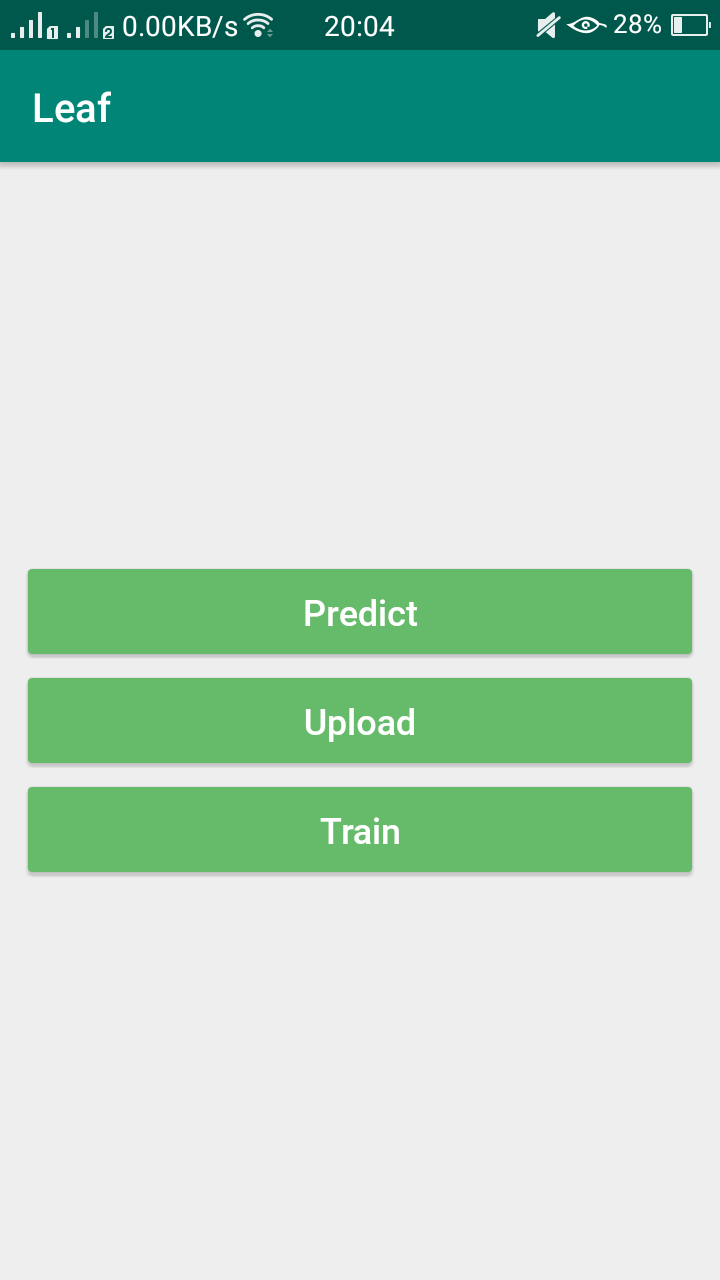
\includegraphics[width=0.7\textwidth]{bab4/figures/main.png}
	\caption{Tampilan awal}
	\label{fig:main}
\end{figure}
\subsection{Implementasi Kelas UploadActivity}
\par Pada kelas UploadActivity pengguna dapat mengunggah gambar beberapa kali dengan nama daun tertentu. Dengan adanya unggahan dari pengguna maka dataset akan bertambah.

\begin{lstlisting}[language=Java, caption=Implementasi Fitur Upload, label=code:upload, firstnumber=53, breaklines]

public class UploadActivity extends AppCompatActivity {
private static final String LOGGING_TAG = "Upload Activity";
private CameraView cameraView;
private final PermissionsDelegate permissionsDelegate = new PermissionsDelegate(this);
private boolean hasCameraPermission;

private CameraKitEventListener cameradListener;
private Button capture;
private EditText textView;

private Fotoapparat fotoapparat;

@Override
protected void onCreate(Bundle savedInstanceState) {
super.onCreate(savedInstanceState);
setContentView(R.layout.activity_upload);
cameraView = findViewById(R.id.camera_view);
capture = findViewById(R.id.btn_capture);
hasCameraPermission = permissionsDelegate.hasCameraPermission();

if (hasCameraPermission) {
cameraView.setVisibility(View.VISIBLE);
} else {
permissionsDelegate
.requestCameraPermission();
}

fotoapparat = createFotoapparat();
takePictureOnClick();
}
private Fotoapparat createFotoapparat() {
return Fotoapparat
.with(this)
.into(cameraView)
.previewScaleType(ScaleType.CenterCrop)
.lensPosition(back())
.logger(loggers(
logcat(),
fileLogger(this)
))
.cameraErrorCallback(new CameraErrorListener() {
@Override
public void onError(CameraException e) {
Toast.makeText(UploadActivity.this, e.toString(), Toast.LENGTH_LONG).show();
}
})
.build();
}

private void takePictureOnClick() {
capture.setOnClickListener(new View.OnClickListener() {
@RequiresApi(api = Build.VERSION_CODES.FROYO)
@Override
public void onClick(View v) {
takePicture();
}
});
}

@RequiresApi(api = Build.VERSION_CODES.FROYO)
private void takePicture() {
PhotoResult photoResult = fotoapparat.takePicture();

photoResult.saveToFile(new File(
getExternalFilesDir("photos"),
"photo.jpg"
));

photoResult
.toBitmap(scaled(0.25f))
.whenDone(new WhenDoneListener<BitmapPhoto>() {
@Override
public void whenDone(@Nullable BitmapPhoto bitmapPhoto) {
if (bitmapPhoto == null) {
Log.e(LOGGING_TAG, "Couldn't capture photo.");
return;
}
Log.d("cek", "whenDone: "+bitmapPhoto);
ImageView imageView = findViewById(R.id.gambar);
Bitmap bitmap1 = RotateBitmap(bitmapPhoto.bitmap,
-bitmapPhoto.rotationDegrees+180);
bitmap1 = flip(bitmap1);
send(bitmap1);
}
});
}


public static Bitmap RotateBitmap(Bitmap source, float angle) {
Matrix matrix = new Matrix();
matrix.postRotate(angle);
return Bitmap.createBitmap(source, 0, 0, source.getWidth(), source.getHeight(), matrix, true);
}

public Bitmap flip(Bitmap bitmap) {
Bitmap bOutput;
Matrix matrix = new Matrix();
matrix.preScale(1.0f, -1.0f);
bOutput = Bitmap.createBitmap(bitmap, 0, 0, bitmap.getWidth(), bitmap.getHeight(), matrix, true);
return bOutput;
}

public void send(Bitmap bitmap) {
Bitmap result = Bitmap.createScaledBitmap(bitmap, 96,96, true);
textView = (EditText) findViewById(R.id.name);
String name = textView.getText().toString();
String myBase64Image = Constans.encodeToBase64(result, Bitmap.CompressFormat.JPEG, 100);
ApiClientAttendance api = Server.builder()
.create(ApiClientAttendance.class);
Call<ResponseApi> upload = api.upload(name,
 "data:image/jpeg;base64,"+myBase64Image);

final SweetAlertDialog pDialog = new SweetAlertDialog(UploadActivity.this, SweetAlertDialog.PROGRESS_TYPE);
pDialog.getProgressHelper()
.setBarColor(Color.parseColor("#A5DC86"));
pDialog.setTitleText("Loading");
pDialog.setCancelable(false);
pDialog.show();

upload.enqueue(new Callback<ResponseApi>() {
@Override
public void onResponse(Call<ResponseApi> call, Response<ResponseApi> response) {
if (response.code() == 200) {
pDialog.dismiss();
new SweetAlertDialog(UploadActivity.this, SweetAlertDialog.SUCCESS_TYPE)
.setTitleText("Hasil")
.setContentText(response.body().getMsg())
.setConfirmText("OK")
.setConfirmClickListener(new SweetAlertDialog.OnSweetClickListener() {
@Override
public void onClick(SweetAlertDialog sDialog) {
sDialog.dismiss();
}
}).show();
} else {
pDialog.dismiss();
new SweetAlertDialog(UploadActivity.this, SweetAlertDialog.WARNING_TYPE)
.setTitleText("Error")
.setContentText("Terjadi kesalahan, mohon ulangi lagi.")
.setConfirmText("OK")
.setConfirmClickListener(new SweetAlertDialog.OnSweetClickListener() {
@Override
public void onClick(SweetAlertDialog sDialog) {
sDialog.dismiss();
}
}).show();
}
}

@Override
public void onFailure(Call<ResponseApi> call, Throwable t) {
pDialog.dismiss();
new SweetAlertDialog(UploadActivity.this, SweetAlertDialog.ERROR_TYPE)
.setTitleText("Hasil")
.setContentText("Internet Anda Bermasalah")
.setConfirmText("OK")
.setConfirmClickListener(new SweetAlertDialog.OnSweetClickListener() {
@Override
public void onClick(SweetAlertDialog sDialog) {
sDialog.dismissWithAnimation();
}
}).show();
System.out.println(t);
}
});
}

@Override
protected void onStart() {
super.onStart();
if (hasCameraPermission) {
fotoapparat.start();
}
}

@Override
protected void onStop() {
super.onStop();
if (hasCameraPermission) {
fotoapparat.stop();
}
}

@Override
public void onRequestPermissionsResult(int requestCode,
@NonNull String[] permissions,
@NonNull int[] grantResults) {
super.onRequestPermissionsResult(
requestCode, permissions, grantResults);
if (permissionsDelegate.resultGranted(
requestCode, permissions, grantResults)) {
hasCameraPermission = true;
fotoapparat.start();
cameraView.setVisibility(View.VISIBLE);
}
}
}
\end{lstlisting}

\par Fitur Upload menggunakan library \textit{fotoapparat} untuk membuka kamera pada ponsel. Gambar yang ditangkap akan diubah dalam bentuk string sebelum dikirim ke server. Untuk mengirim data ke server digunakan library Retrofit2.

\par Berikut adalah tampilan dari laman upload.
\begin{figure}[H]
	\centering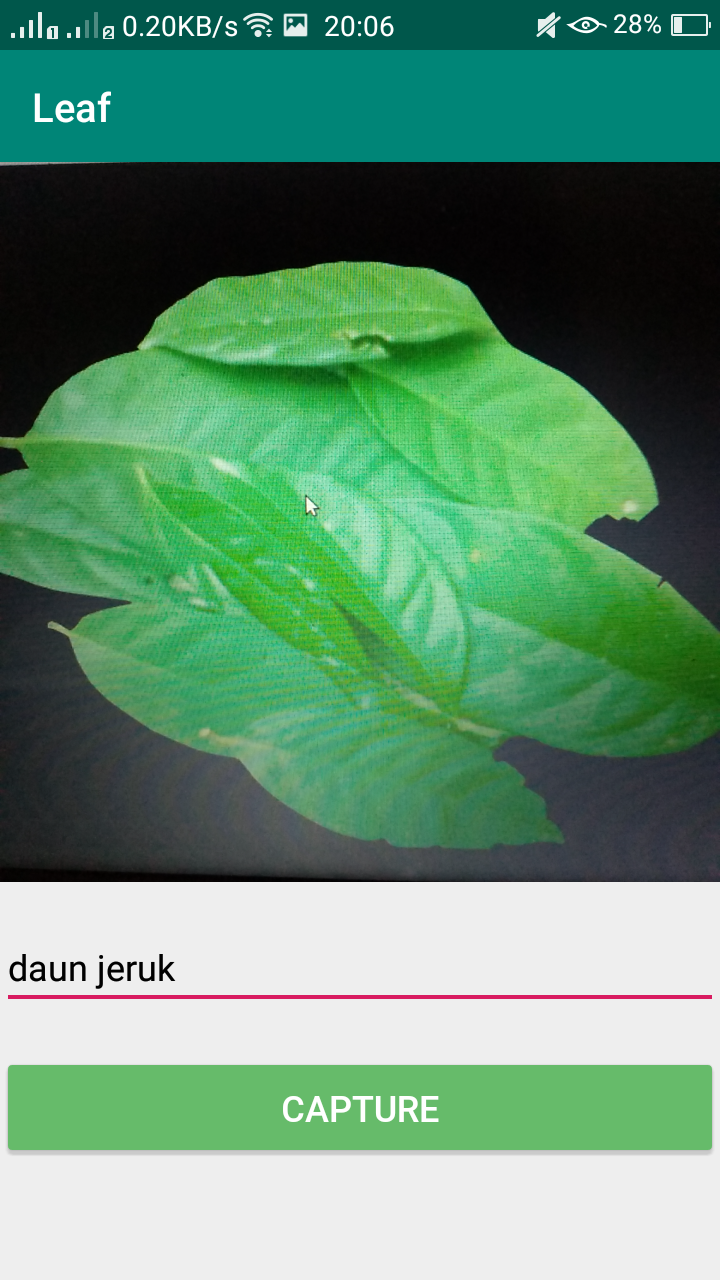
\includegraphics[width=0.7\textwidth]{bab4/figures/upload.png}
	\caption{Tampilan Upload}
	\label{fig:upload}
\end{figure}
\subsection{Implementasi Kelas PredictActivity}
\begin{lstlisting}[language=Java, caption=Implementasi Kelas PredictActivity, label=code:predict, firstnumber=48]
public class PredictActivity extends AppCompatActivity {
private static final String LOGGING_TAG = "New Predict Activity";

private final PermissionsDelegate permissionsDelegate = new PermissionsDelegate(this);
private boolean hasCameraPermission;
private RelativeLayout cameraLayout;
private CameraView cameraView;
private Button capture;
private Fotoapparat fotoapparat;

@Override
protected void onCreate(Bundle savedInstanceState) {
super.onCreate(savedInstanceState);
setContentView(R.layout.activity_predict);

cameraLayout = findViewById(R.id.CameraLayout);
cameraView = findViewById(R.id.camera_view);
capture = findViewById(R.id.btn_capture);
hasCameraPermission = permissionsDelegate.hasCameraPermission();


cameraLayout.getLayoutParams().height = cameraLayout.getLayoutParams().width;

if (hasCameraPermission) {
cameraView.setVisibility(View.VISIBLE);
} else {
permissionsDelegate.requestCameraPermission();
}

fotoapparat = createFotoapparat();
takePictureOnClick();
}

private Fotoapparat createFotoapparat() {
return Fotoapparat
.with(this)
.into(cameraView)
.previewScaleType(ScaleType.CenterCrop)
.lensPosition(back())
.logger(loggers(
logcat(),
fileLogger(this)
))
.cameraErrorCallback(new CameraErrorListener() {
@Override
public void onError(@NotNull CameraException e) {
Toast.makeText(PredictActivity.this, e.toString(), Toast.LENGTH_LONG).show();
}
})
.build();
}

private void takePictureOnClick() {
capture.setOnClickListener(new View.OnClickListener() {
@RequiresApi(api = Build.VERSION_CODES.FROYO)
@Override
public void onClick(View v) {
takePicture();
}
});
}

@RequiresApi(api = Build.VERSION_CODES.FROYO)
private void takePicture() {
PhotoResult photoResult = fotoapparat.takePicture();

photoResult.saveToFile(new File(
getExternalFilesDir("photos"),
"photo.jpg"
));

photoResult
.toBitmap(scaled(0.25f))
.whenDone(new WhenDoneListener<BitmapPhoto>() {
@Override
public void whenDone(@Nullable BitmapPhoto bitmapPhoto) {
if (bitmapPhoto == null) {
Log.e(LOGGING\_TAG, "Couldn't capture photo.");
return;
}
Log.d("cek", "whenDone: " + bitmapPhoto);
ImageView imageView = findViewById(R.id.gambar);
Bitmap bitmap1 = RotateBitmap(bitmapPhoto.bitmap, -bitmapPhoto.rotationDegrees + 180);
bitmap1 = flip(bitmap1);
send(bitmap1);
}
});
}

public static Bitmap RotateBitmap(Bitmap source, float angle) {
Matrix matrix = new Matrix();
matrix.postRotate(angle);
return Bitmap.createBitmap(source, 0, 0, source.getWidth(), source.getHeight(), matrix, true);
}

public Bitmap flip(Bitmap bitmap) {
Bitmap bOutput;
Matrix matrix = new Matrix();
matrix.preScale(1.0f, -1.0f);
bOutput = Bitmap.createBitmap(bitmap, 0, 0, bitmap.getWidth(), bitmap.getHeight(), matrix, true);
return bOutput;
}

@Override
protected void onStart() {
super.onStart();
if (hasCameraPermission) {
fotoapparat.start();
}
}

@Override
protected void onStop() {
super.onStop();
if (hasCameraPermission) {
fotoapparat.stop();
}
}

@Override
public void onRequestPermissionsResult(int requestCode,
@NonNull String[] permissions,
@NonNull int[] grantResults) {
super.onRequestPermissionsResult(
requestCode, permissions, grantResults);
if (permissionsDelegate.resultGranted(
requestCode, permissions, grantResults)) {
hasCameraPermission = true;
fotoapparat.start();
cameraView.setVisibility(View.VISIBLE);
}
}

public void send(Bitmap bitmap) {
Bitmap result = Bitmap.createScaledBitmap(bitmap, 96, 96, true);
String myBase64Image = Constans.encodeToBase64(result, Bitmap.CompressFormat.JPEG, 100);

Call<ResponseApi> predict;
ApiClientAttendance api = Server.builder()
.create(ApiClientAttendance.class);
predict = api.predict("data:image/jpeg;base64," + myBase64Image);

final SweetAlertDialog pDialog = new SweetAlertDialog(PredictActivity.this, SweetAlertDialog.PROGRESS_TYPE);
pDialog.getProgressHelper()
.setBarColor(Color.parseColor("#A5DC86"));
pDialog.setTitleText("Loading");
pDialog.setCancelable(false);
pDialog.show();

predict.enqueue(new Callback<ResponseApi>() {
@Override
public void onResponse(Call<ResponseApi> call, Response<ResponseApi> response) {
if (response.code() == 200) {
pDialog.dismiss();

String r = response.body().getMsg();
String[] result = r.trim().split(",");

if (result[0].equals("ACCEPTED")) {
new SweetAlertDialog(PredictActivity.this, SweetAlertDialog.SUCCESS_TYPE)
.setTitleText("Hasil")
.setContentText(response.body().getMsg())
.setConfirmText("OK")
.setConfirmClickListener(new SweetAlertDialog.OnSweetClickListener() {
@Override
public void onClick(SweetAlertDialog sDialog) {
sDialog.dismiss();
}
}).show();
} else {
new SweetAlertDialog(PredictActivity.this, SweetAlertDialog.WARNING_TYPE)
.setTitleText("Error")
.setContentText(response.body().getMsg())
.setConfirmText("OK")
.setConfirmClickListener(new SweetAlertDialog.OnSweetClickListener() {
@Override
public void onClick(SweetAlertDialog sDialog) {
sDialog.dismiss();
}
}).show();
}
} else {
pDialog.dismiss();
new SweetAlertDialog(PredictActivity.this, SweetAlertDialog.WARNING_TYPE)
.setTitleText("Error")
.setContentText("Terjadi kesalahan, mohon ulangi kembali.")
.setConfirmText("OK")
.setConfirmClickListener(new SweetAlertDialog.OnSweetClickListener() {
@Override
public void onClick(SweetAlertDialog sDialog) {
sDialog.dismiss();
}
}).show();
}
}

@Override
public void onFailure(Call<ResponseApi> call, Throwable t) {
pDialog.dismiss();
new SweetAlertDialog(PredictActivity.this, SweetAlertDialog.ERROR_TYPE)
.setTitleText("Error")
.setContentText("Terdapat masalah dengan koneksi anda, mohon ulangi kembali.")
.setConfirmText("OK")
.setConfirmClickListener(new SweetAlertDialog.OnSweetClickListener() {
@Override
public void onClick(SweetAlertDialog sDialog) {
sDialog.dismissWithAnimation();
}
}).show();
}
});
}
}
\end{lstlisting}

\par Kelas PredictActivity mirip seperti kelas UploadActivity dalam hal tampilan, bedanya adalah kelas ini ketika menembak API pada server akan mendapatkan response berupa nama daun yang diprediksi. Tampilan dari fitur Predict adalah sebagai berikut.
\begin{figure}[H]
	\centering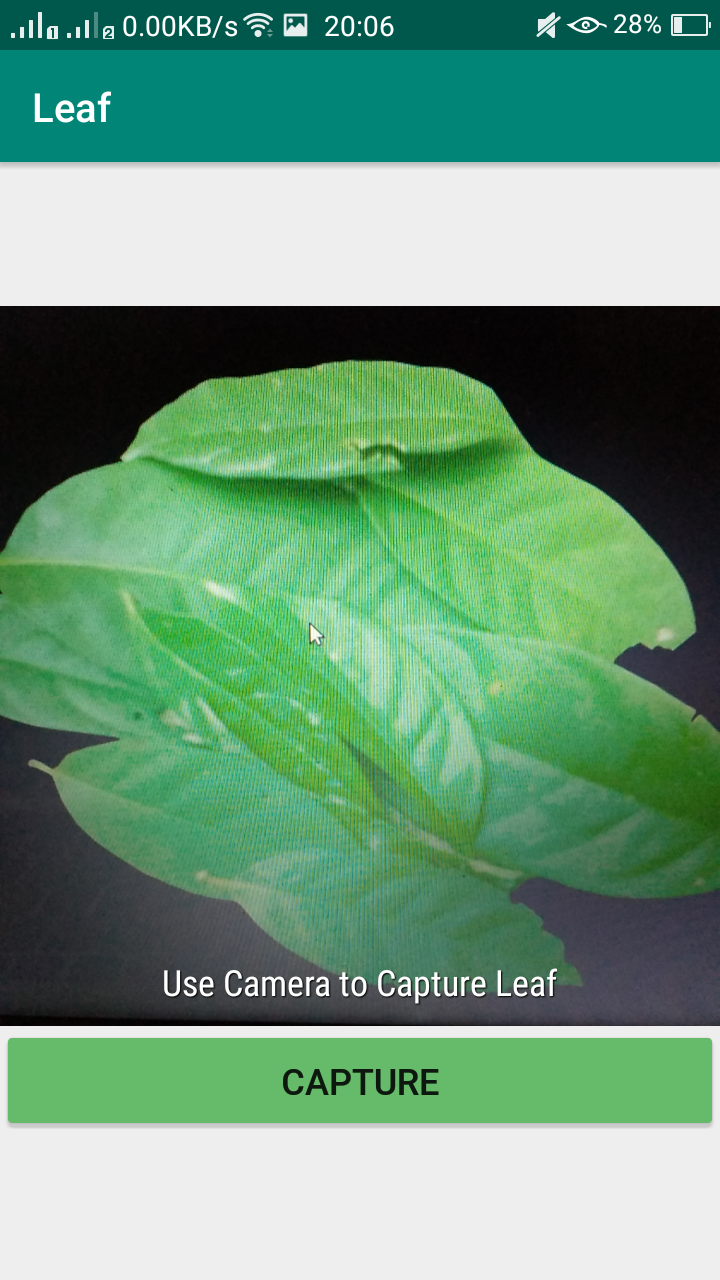
\includegraphics[width=0.7\textwidth]{bab4/figures/predict.png}
	\caption{Tampilan Predict}
	\label{fig:predict}
\end{figure}
\subsection{API}
\par Berikut adalah sumber kode untuk memanggil API pada server.

\begin{lstlisting}[language=python, caption=Pemanggilan API menggunakan Retrofit2, label=code:api, firstnumber=0]
public interface ApiClientAttendance {
@FormUrlEncoded
@POST("/upload/")
Call<ResponseApi> upload(@Field("name") String name,
@Field("image") String image);

@POST("/train/")
Call<ResponseApi> train();

@FormUrlEncoded
@POST("/predict/")
Call<ResponseApi> predict(@Field("image") String image);
}
\end{lstlisting} \cleardoublepage
	\chapter{UJI COBA DAN EVALUASI}
Pada bab ini akan dijelaskan tentang uji coba dan evaluasi dari implementasi sistem yang telah dilakukan pada bab 4.

\section{Lingkungan Uji Coba}
Lingkungan uji coba menggunakan sebuah komputer dengan spesifikasi perangkat keras dan perangkat lunak sebagai berikut.

\begin{enumerate}
	\item Perangkat Keras
	\begin{enumerate}
		\item GPU: 1x Tesla K80 , having 2496 CUDA cores, compute 3.7, 12GB(11.439GB Usable) GDDR5 VRAM.
		\item CPU: 1x single core hyper threaded i.e(1 core, 2 threads) Xeon Processors @2.3Ghz (No Turbo Boost) , 45 MB Cache.
	\end{enumerate}
	\item Perangkat Lunak
	\begin{enumerate}
		\item Sistem Operasi Linux Ubuntu 1804 64-bit
		\item Android Studio
		\item Bahasa Pemrograman Java
		\item Bahasa Pemrograman Python
		\item Library Keras
	\end{enumerate}
\end{enumerate}

\section{Dataset}
\par Dataset yang digunakan adalah dataset daun dari \url{https://archive.ics.uci.edu/ml/datasets/leaf}. Dataset ditambahkan dengan dataset dari penulis sendiri. Dataset akan dipecah dengan rasio 7 : 3 untuk data train dan data test. 

\section{Uji Coba Ekstraksi Fitur Menggunakan Pre-Trained Model}

\par Hasil dari evaluasi pembuatan model yang diekstraksi dengan \textit{pre-trained model} yang disediakan adalah :


\begin{table}[ht]
	\centering
	\begin{tabularx}{1.0\textwidth}
		{|p{2cm}|X|X|X|X|}
	\hline
	\rowcolor{lightgray} \centering Model&Rank-1&Precision&Recall&F1 Score \\ \hline
	\centering VGG16	& 	95.62 & 	97.0	& 96.0	&	95.0 \\ \hline
	\centering VGG19	& 94.89 &	96.0	&95.0	& 94.0 \\ \hline
    \rowcolor{green} \centering MobileNet	&	96.35	& 97.0	& 96.0 &	96.0 \\ \hline
	\centering ResNet50	& 53.28	& 61.0	& 53.0	& 51.0 \\ \hline
	\centering InceptionV3	&	93.43	&  95.0 & 93.0 & 93.0 \\ \hline
	\centering Xception	&	93.43	& 95.0 & 93.0 & 93.0 \\ \hline
	\end{tabularx}
	\caption{Tabel data hasil evaluasi model}
	\label{table:hasil}
\end{table}

\begin{table}[ht]
	\centering
	\begin{tabularx}{1.0\textwidth}
		{|X|X|}
		\hline
		\rowcolor{lightgray} \centering Model& Waktu Ekstraksi Fitur \\ \hline
		\centering VGG16	& 	8 menit 56 detik \\ \hline
		\centering VGG19	& 10 menit 3 detik \\ \hline
		\rowcolor{green} \centering MobileNet	&	2 menit 5 detik \\ \hline
		\centering ResNet50	& 15 menit 27 detik	\\ \hline
		\centering InceptionV3	&	6 menit \\ \hline
		\centering Xception	&	5 menit 38 detik \\ \hline
	\end{tabularx}
	\caption{Tabel data waktu ekstraksi fitur}
	\label{table:hasil}
\end{table}

Dari hasil tersebut, dapat disimpulkan bahwa arsitektur yang optimal dalam pengklasifikasian jenis daun adalah MobileNet. MobileNet memiliki akurasi paling tinggi, 96.35\% dan waktu ekstraksi fitur paling cepat yaitu 2 menit 5 detik.

\section{Hasil dari Aplikasi}
Berikut adalah hasil tangkapan layar dari aplikasi :

\begin{figure}[ht]
\begin{subfigure}{0.5\textwidth}
	\centering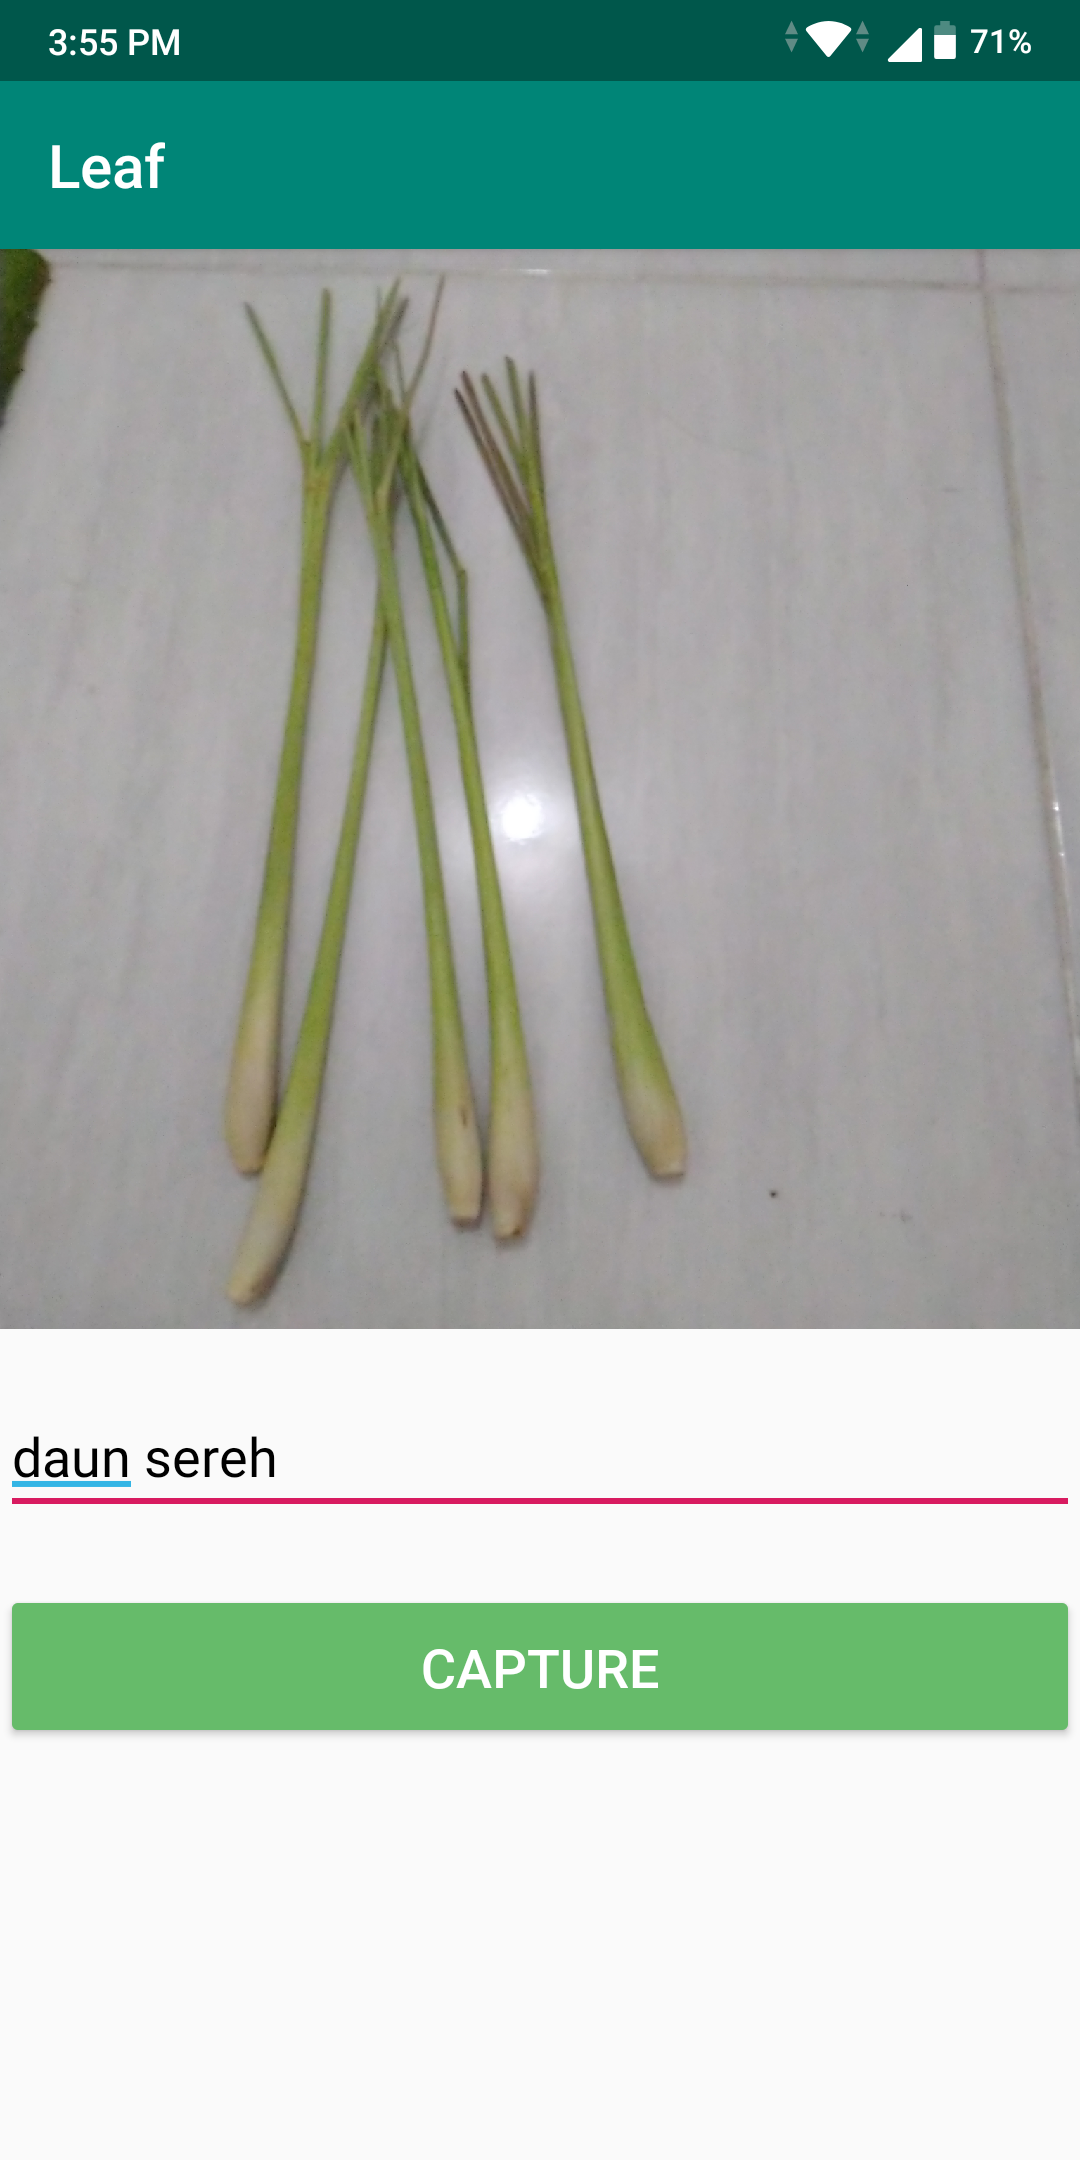
\includegraphics[width=\linewidth]{bab5/figures/uploadsereh.png}
	\caption{Fungsi Upload}
	\label{fig:analisis_label_a}
\end{subfigure}
~
\begin{subfigure}{0.5\textwidth}
	\centering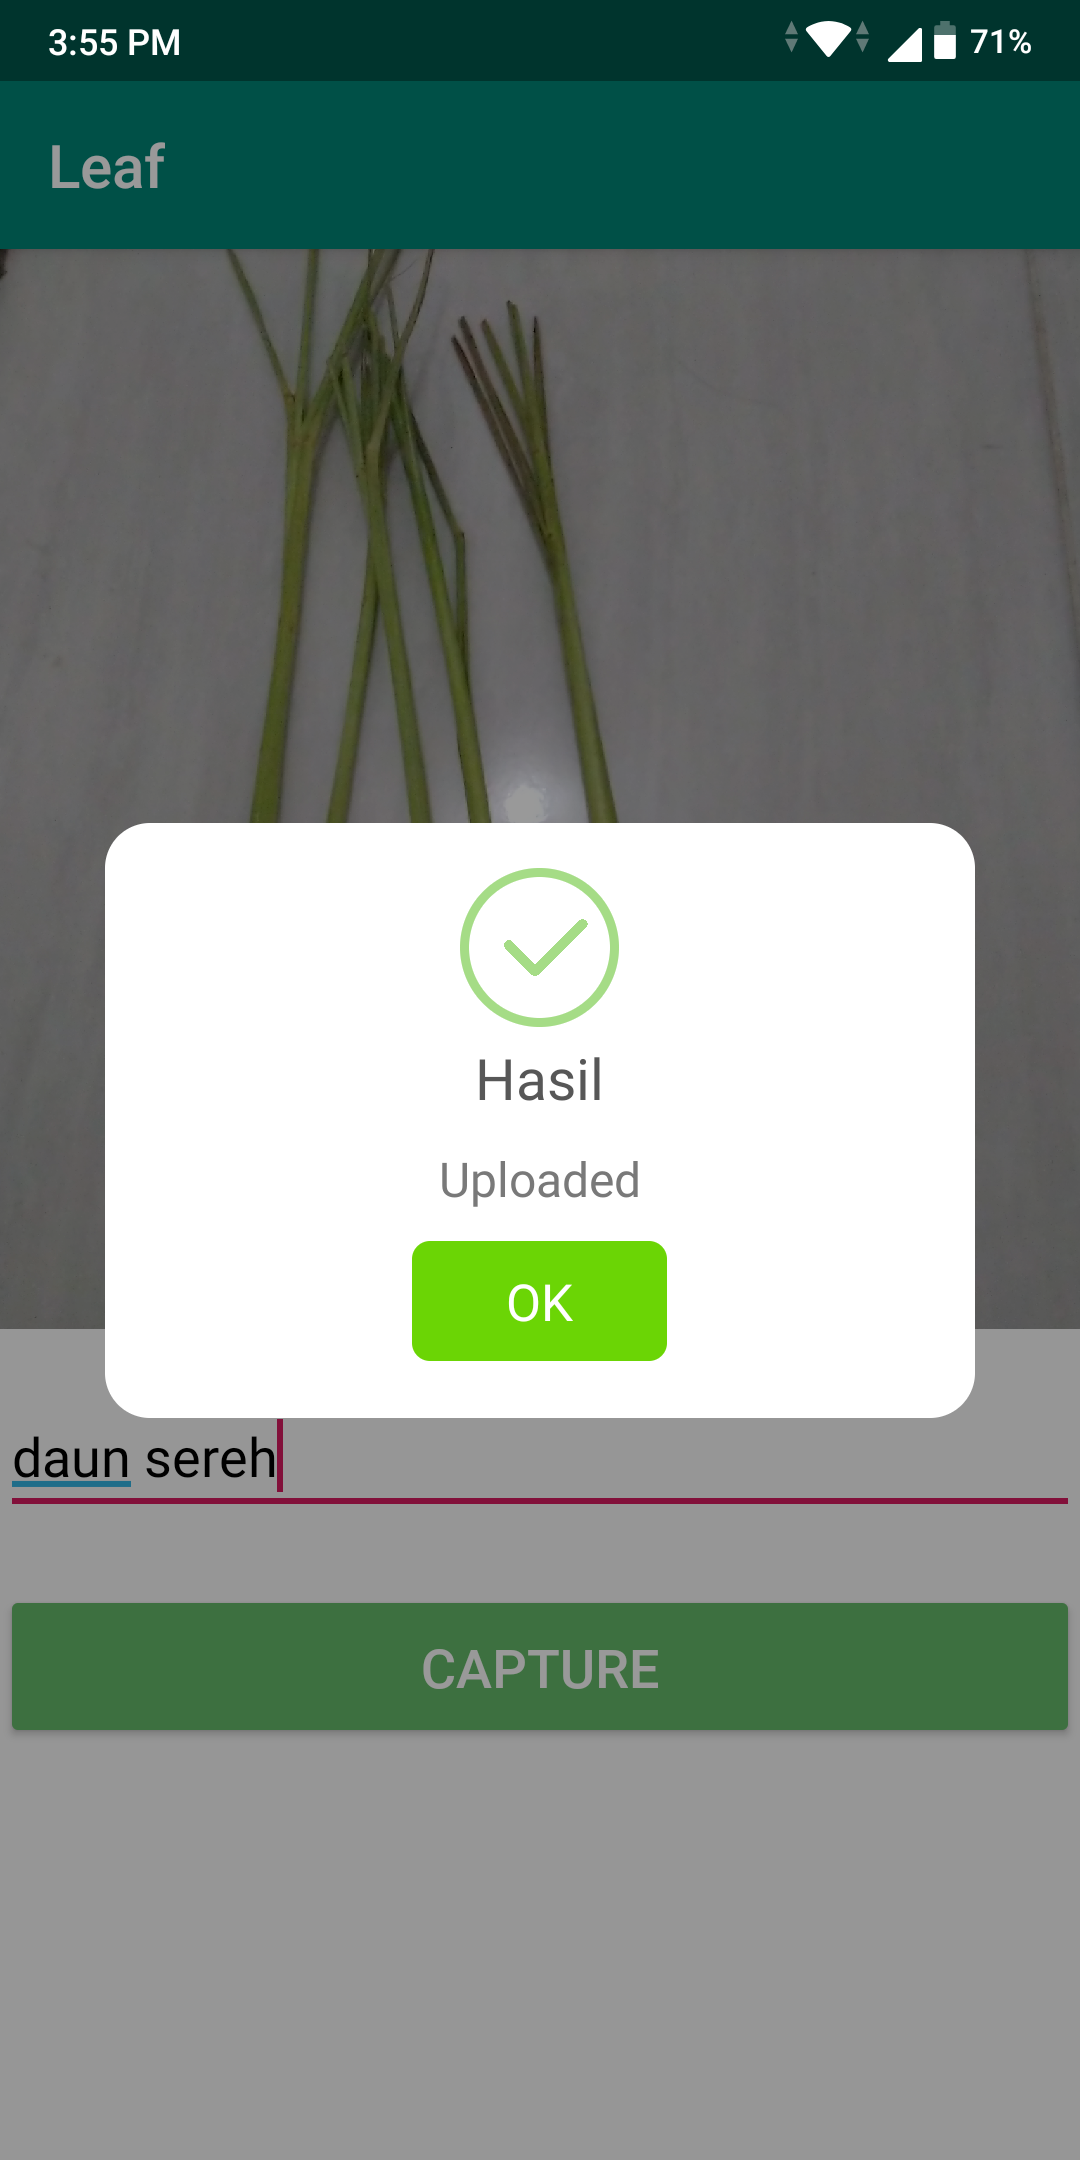
\includegraphics[width=\linewidth]{bab5/figures/uploaded.png}
	\caption{Berhasil Upload}
	\label{fig:analisis_label_b}
\end{subfigure}
\caption{Hasil tangkap layar pada fitur Upload}
\end{figure}

\begin{figure}[ht]
	\centering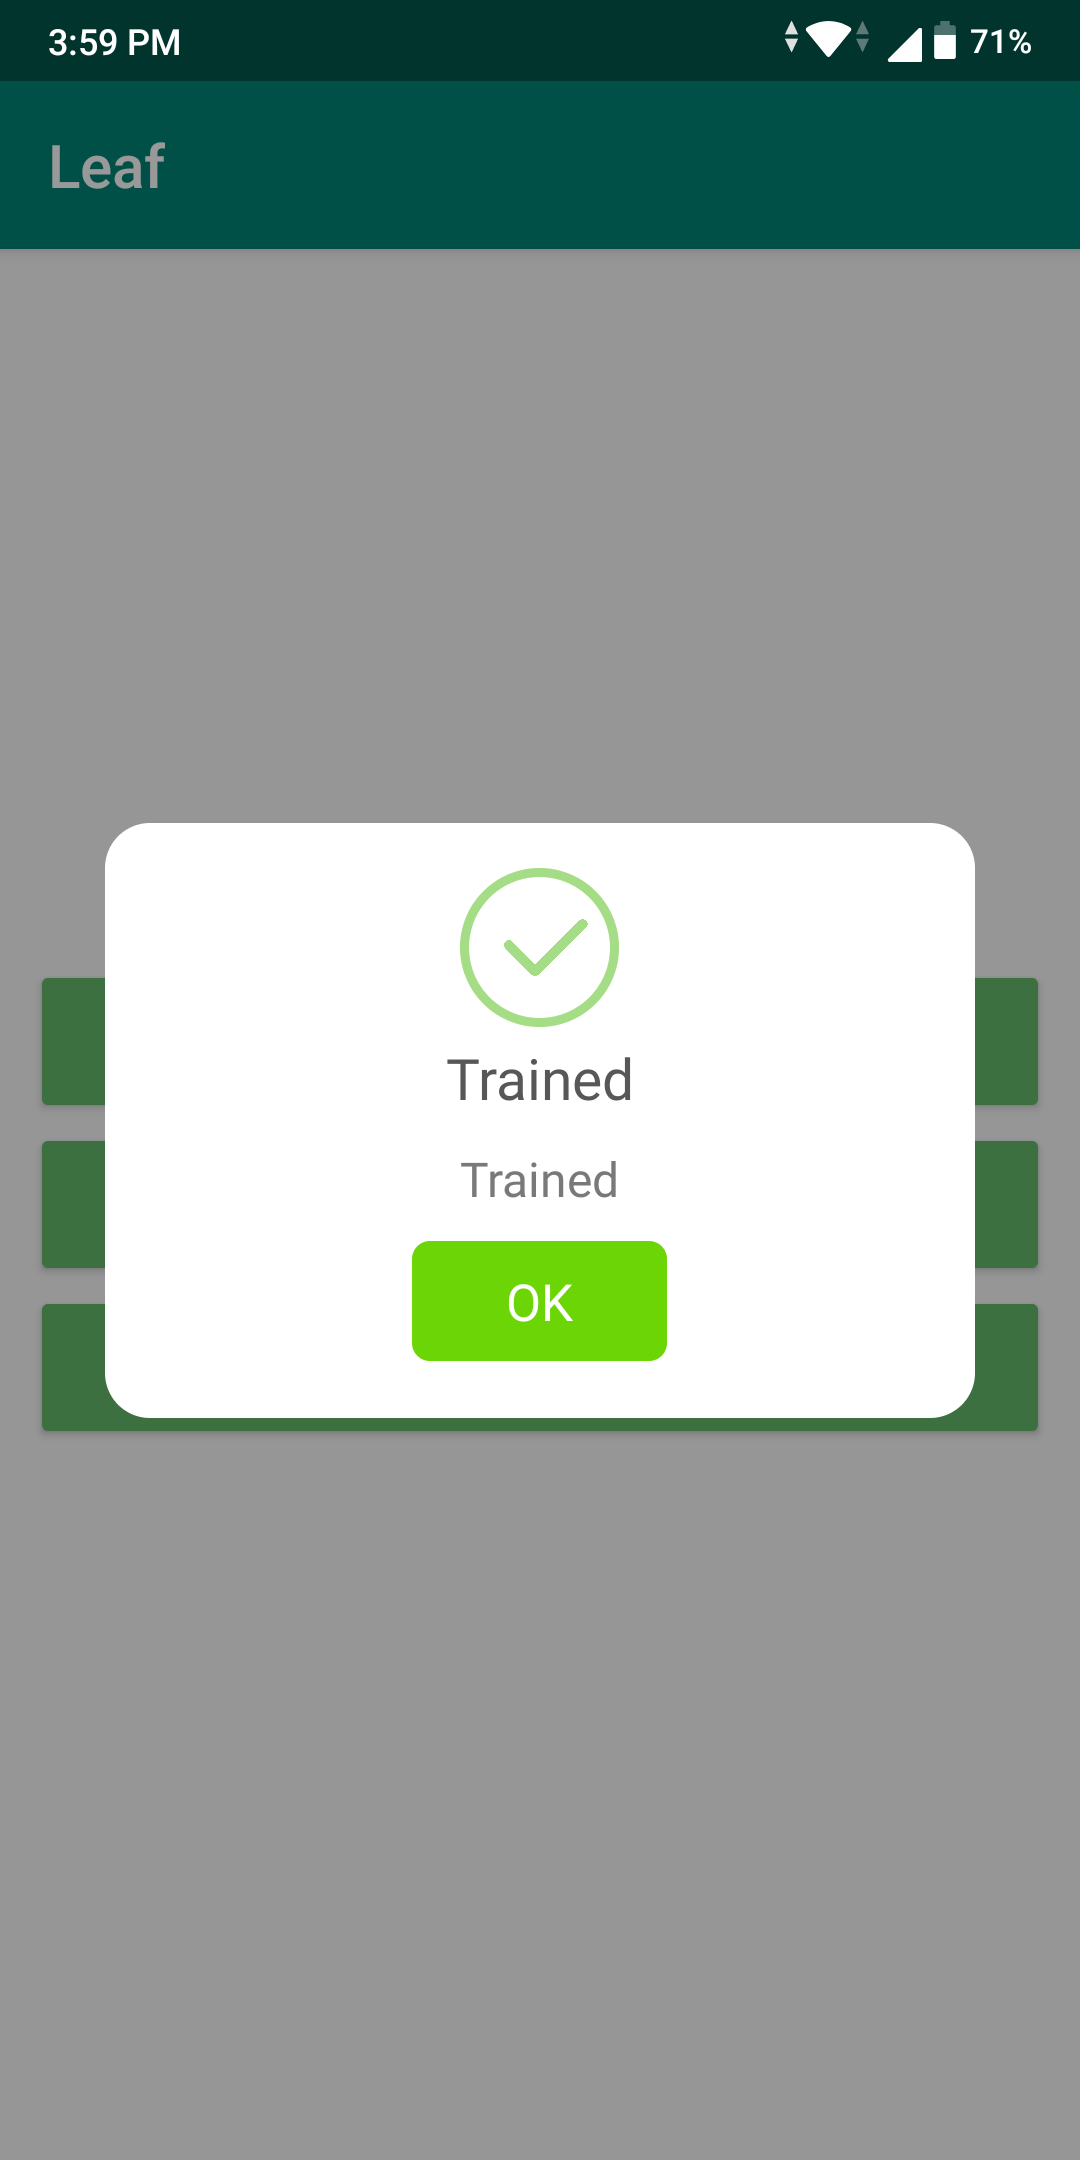
\includegraphics[width=0.5\textwidth]{bab5/figures/trained.png}
	\caption{Berhasil Train}
	\label{fig:train}
\end{figure}

\begin{figure}[ht]
	\begin{subfigure}{0.5\textwidth}
		\centering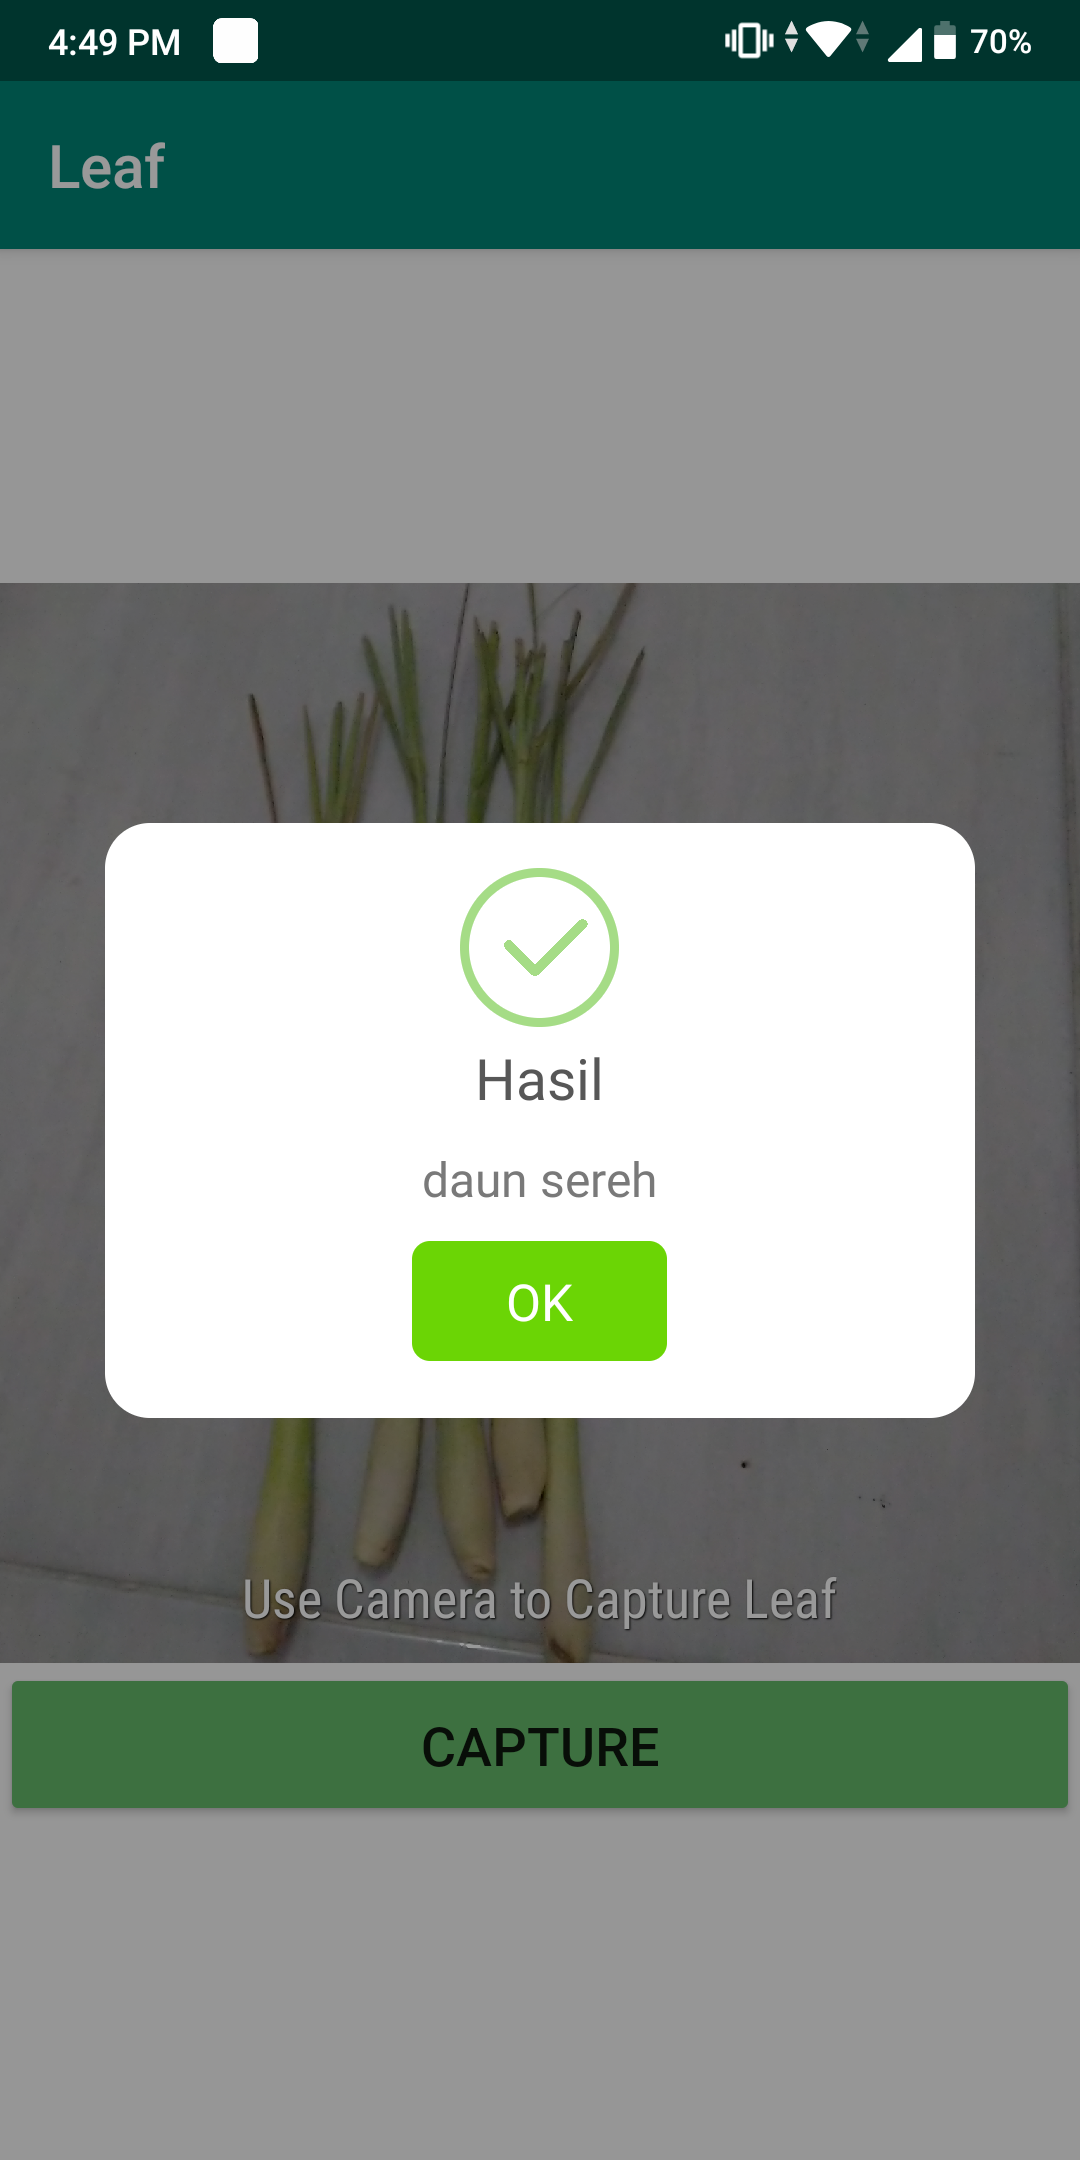
\includegraphics[width=\linewidth]{bab5/figures/ss2hasil.png}
		\caption{Hasil Prediksi Daun Sereh}
		\label{fig:hasil2}
	\end{subfigure}
	~
	\begin{subfigure}{0.5\textwidth}
		\centering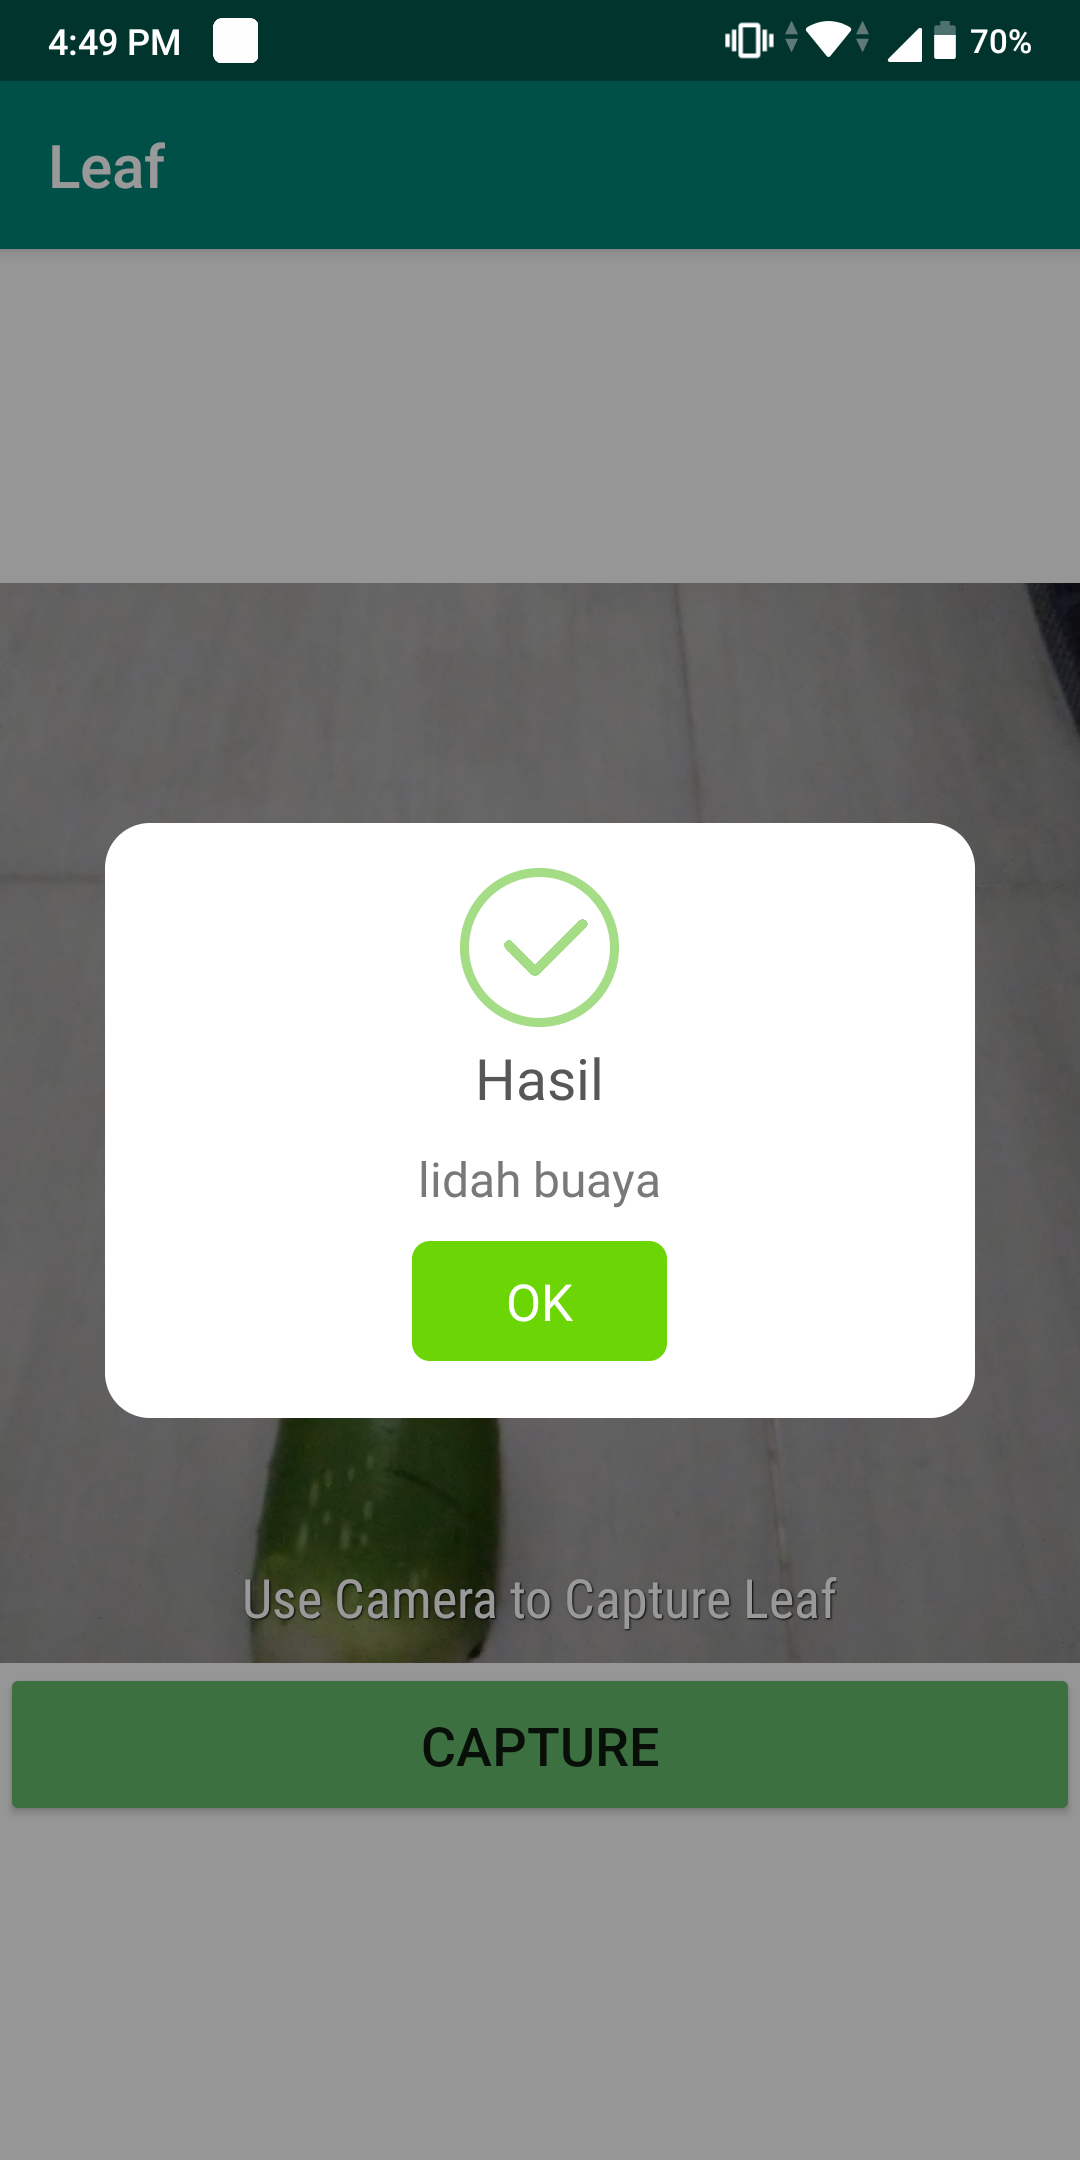
\includegraphics[width=\linewidth]{bab5/figures/ss1hasil.png}
		\caption{Hasil Prediksi Daun Lidah Buaya}
		\label{fig:hasil1}
	\end{subfigure}
\caption{Hasil tangkap layar pada fitur Predict}
\end{figure}

\begin{table}[ht]
	\centering
	\begin{tabularx}{1.0\textwidth}
		{|X|X|}
		\hline
		\rowcolor{lightgray} \centering Nama Daun& Hasil Benar dari 10 Pengujian\\ \hline
		\centering Lidah Buaya	& 	10 \\ \hline
		\centering Sereh	& 10  \\ \hline
		\centering Daun Jeruk	&	9 \\ \hline
		\centering Daun Beluntas	& 7	\\ \hline
	\end{tabularx}
	\caption{Tabel hasil pengujian pada daun}
	\label{table:hasil}
\end{table}


 \cleardoublepage
	\chapter{KESIMPULAN DAN SARAN}
Bab ini membahas tentang kesimpulan yang didasari oleh hasil uji coba yang telah dilakukan pada bab sebelumnya. Kesimpulan nantinya sebagai jawaban dari rumusan masalah yang dikemukakan. Selain kesimpulan, juga terdapat saran yang ditujukan untuk pengembangan penelitian lebih lanjut di masa depan.

\section{Kesimpulan}
Dalam pengerjaan Tugas Akhir ini setelah melalui tahap perancangan aplikasi, implementasi metode, serta uji coba, diperoleh kesimpulan sebagai berikut:

\begin{enumerate}
	\item Untuk mengimplementasi \textit{transfer learning} untuk mendeteksi daun digunakan library Keras dan pengimplementasian ekstraksi fitur menggunakan model yang tersedia.
	\item Untuk mengembangkan aplikasi pendeteksi daun berbasis Android yang mengirim gambar ke server dan menerima balasan berupa jenis daun diterapkan REST API untuk memanggil server yang kemudian akan mengirim balasan ke Android. Untuk memanggil server digunakan Retrofit2.
	\item Untuk melakukan proses klasifikasi daun pada server, digunakan model yang telah disimpan. Model dibuat dengan menggunakan \textit{transfer knowledge} dari model-model yang sudah disediakan Keras.
	\item Arsitektur yang paling akurat dalam mendeteksi daun menggunakan Logistic Regression adalah MobileNet, dengan akurasi 96\%.
\end{enumerate}

\section{Saran}
Berikut merupakan beberapa saran untuk pengembangan sistem di masa yang akan datang. Saran-saran ini didasarkan pada hasil perancangan, implementasi, dan uji coba yang telah dilakukan.
\begin{enumerate}
	\item Diperlukan hardware yang mumpuni untuk melatih model.
	\item Memperbaiki desain pada aplikasi Android, termasuk pemilihan warna dan tata letak.
	\item Membuat tombol "Bantuan" untuk mempermudah pengguna.
\end{enumerate} \cleardoublepage
	
	\backmatter
	\printbibliography
	\chapter{LAMPIRAN A: MainActivity}
\begin{lstlisting}[language=Java, caption=Implementasi Kelas Main, label=code:main, firstnumber=23]
public class MainActivity extends AppCompatActivity {
Button predict;
Button train;
Button upload;
@Override
protected void onCreate(Bundle savedInstanceState) {
super.onCreate(savedInstanceState);
setContentView(R.layout.activity_main);
predict = (Button) findViewById(R.id.predict);

// Capture button clicks
predict.setOnClickListener(new View.OnClickListener() {
public void onClick(View arg0) {

// Start NewActivity.class
Intent myIntent = new Intent(MainActivity.this,
PredictActivity.class);
System.out.println("predict");
startActivity(myIntent);
}
});

upload = (Button) findViewById(R.id.upload);

// Capture button clicks
upload.setOnClickListener(new View.OnClickListener() {
public void onClick(View arg0) {

// Start NewActivity.class
Intent myIntent = new Intent(MainActivity.this,
UploadActivity.class);
System.out.println("uploaded");
startActivity(myIntent);
}
});

train = (Button) findViewById(R.id.train);
train.setOnClickListener(new View.OnClickListener() {
@Override
public void onClick(View v) {
ApiClientAttendance api = Server.builder()
.create(ApiClientAttendance.class);
Call<ResponseApi> train = api.train();
System.out.println("trained");
final SweetAlertDialog pDialog = new SweetAlertDialog(MainActivity.this, SweetAlertDialog.PROGRESS_TYPE);
pDialog.getProgressHelper().
setBarColor(Color.parseColor("#A5DC86"));
pDialog.setTitleText("Loading");
pDialog.setCancelable(false);
pDialog.show();

train.enqueue(new Callback<ResponseApi>() {
@Override
public void onResponse(Call<ResponseApi> call, Response<ResponseApi> response) {
if (response.code() == 200) {
pDialog.dismiss();
new SweetAlertDialog(MainActivity.this, SweetAlertDialog.SUCCESS_TYPE)
.setTitleText("Trained")
.setContentText(response.body().getMsg())
.setConfirmText("OK")
.setConfirmClickListener(new SweetAlertDialog.OnSweetClickListener() {
@Override
public void onClick(SweetAlertDialog sDialog) {
sDialog.dismiss();
}
}).show();
} else {
pDialog.dismiss();
new SweetAlertDialog(MainActivity.this, SweetAlertDialog.WARNING_TYPE)
.setTitleText("Error")
.setContentText("Terjadi kesalahan, mohon ulangi lagi.")
.setConfirmText("OK")
.setConfirmClickListener(new SweetAlertDialog.OnSweetClickListener() {
@Override
public void onClick(SweetAlertDialog sDialog) {
sDialog.dismiss();
}
}).show();
}
}

@Override
public void onFailure(Call<ResponseApi> call, Throwable t) {
pDialog.dismiss();
new SweetAlertDialog(MainActivity.this, SweetAlertDialog.ERROR_TYPE)
.setTitleText("Hasil")
.setContentText("Internet Anda Bermasalah")
.setConfirmText("OK")
.setConfirmClickListener(new SweetAlertDialog.OnSweetClickListener() {
@Override
public void onClick(SweetAlertDialog sDialog) {
sDialog.dismissWithAnimation();
}
}).show();
System.out.println(t);
}
});
}
});
cek();
}
}
\end{lstlisting}
	
\chapter{BIODATA PENULIS}

\begin{wrapfigure}{l}{0.3\textwidth}
	
\includegraphics[height=0.25\textheight]{figures/frieda.jpg}
\end{wrapfigure}

Penulis bernama \penulis, lahir di Malang pada tanggal 26 September 1997. Penulis sempat menempuh pendidikan di SDN Cengkareng Barat 012 Pagi, SDN Srengseng 05 Pagi, SMPN 75 Jakarta dari tahun 2009 hingga 2012, SMAN 8 Jakarta dari tahun 2012 sampai dengan 2015 dan sedang menjalani studi di jurusan Informatika di Fakultas Teknologi Informasi Institut Teknologi Sepuluh Nopember.

Di luar kesibukan akademik, penulis cukup aktif dalam organisasi baik dari dalam maupun luar jurusan.
Penulis aktif dalam organisasi dan
kepanitiaan Himpunan Mahasiswa Teknik Computer (HMTC) dan Schematics. Pernah menjadi staf Departemen Teknologi pada HMTC 2016-2017 dan sekretaris National Programming Contest Schematics 2017-2018. Penulis juga aktif dalam perlombaan Competitive Programming dan Developer Camp. 
Selain itu, penulis memiliki pengalaman magang di PT. Karya Anak Bangsa, PT. Nodeflux Teknologi Indonesia, PT. Dynamo Media Network dan PT. Tokopedia. Penulis dapat dihubungi melalui surat elektronik di \href{mailto:hallofrieda@gmail.com}{hallofrieda@gmail.com}.
\end{document}
